\documentclass[12pt,a4paper]{article}

% ---------- XeLaTeX font setup ----------
\usepackage{fontspec}
\setmainfont{Times New Roman}

\usepackage[a4paper,margin=1in]{geometry}
\usepackage{graphicx}
\usepackage{booktabs}
\usepackage{amsmath,amssymb}
\usepackage{float}
\usepackage{xcolor}
\usepackage[hidelinks]{hyperref}
\usepackage{listings}
\usepackage{enumitem}
\usepackage{fancyhdr}
\usepackage{longtable}
\usepackage{caption}

\hypersetup{colorlinks=true,linkcolor=blue,urlcolor=blue}

\pagestyle{fancy}
\fancyhf{}
\lhead{ICS1512}
\rhead{Machine Learning Algorithms Laboratory}
\cfoot{\thepage}

\lstset{
language=Python,
basicstyle=\ttfamily\small,
numbers=left,
frame=single,
breaklines=true,
showstringspaces=false
}

% Path to figures folder (ml_lab/figures/), relative to ml_lab/reports/
\graphicspath{{../figures/}}

\begin{document}

\begin{tabular}{|p{4cm}|p{11cm}|}
\hline
Experiment No. & 3 \\ \hline
Experiment Title & Regression Analysis using Linear and Regularized Models \\ \hline
GitHub Repository & \url{https://github.com/Ray-Audrey/ML-Experiments} \\ \hline
Student Name & Harshita S \\ \hline
Register Number & 3122247001020\\ \hline
Faculty & Dr. Poreddy Ajay Kumar Reddy \\ \hline
Submission Date & 27/07/2026\\ \hline
\end{tabular}

\section{Executive Summary}

This report presents a complete regression analysis pipeline built to predict the \textbf{Loan Sanction Amount (USD)} for customers applying for loans, using a 30{,}000-record Kaggle dataset containing a mix of numerical and categorical financial attributes. Four regression algorithms -- Linear Regression, Ridge Regression, Lasso Regression, and Elastic Net Regression -- were implemented, tuned using 5-fold GridSearchCV, and compared on identical train/test splits. All four models converged to broadly similar performance (test R$^2 \approx 0.60$), which indicates that the dataset's signal is largely linear in nature and dominated by a small number of strong predictors -- namely Loan Amount Request, Property Price, Current Loan Expenses, and Credit Score. Lasso Regression was ultimately selected as the best-performing and most parsimonious model, achieving the lowest RMSE (29{,}903.95) and highest test R$^2$ (0.6024) while also performing implicit feature selection through L1 sparsity.

\section{Objective}

To implement linear and regularized regression models -- Linear Regression, Ridge Regression, Lasso Regression, and Elastic Net Regression -- for predicting a continuous target variable (Loan Sanction Amount), evaluate their performance using multiple metrics, visualize model behavior, and analyze overfitting, underfitting, and bias--variance characteristics. The experiment also involves:

\begin{itemize}
\item Performing structured exploratory data analysis (EDA) to understand feature distributions and relationships.
\item Handling missing values in both numerical and categorical features using appropriate imputation strategies.
\item Encoding categorical features and scaling numerical features to prepare data for linear models.
\item Performing hyperparameter tuning using GridSearchCV with 5-fold cross-validation.
\item Comparing models using MAE, MSE, RMSE, and R$^2$ Score on both validation folds and a held-out test set.
\item Studying how L1 and L2 regularization reshape model coefficients and generalization behavior.
\end{itemize}

\section{Problem Statement}

Loan approval systems require accurate prediction of the sanctioned loan amount based on customer information, financial status, credit history, and property details. Manually assessing every application is time-consuming and prone to inconsistency; a well-calibrated regression model can support underwriters by providing a data-driven estimate of the appropriate sanction amount, which can then be reviewed and adjusted by a human decision-maker.

The objective of this experiment is to develop machine learning regression models that can predict the loan sanction amount for a customer, and to rigorously compare unregularized and regularized variants to understand which best balances predictive accuracy against model complexity and stability.

\textbf{Input:}

The input consists of customer-related features including:
\begin{itemize}
\item Demographic details -- Age, Gender
\item Financial details -- Income, Income Stability, Credit Score, No. of Defaults, Has Active Credit Card
\item Employment details -- Profession, Type of Employment, Location
\item Loan-related details -- Loan Amount Request, Current Loan Expenses, Expense Type 1/2, Dependents, Co-Applicant
\item Property details -- Property Age, Property Type, Property Location, Property Price
\end{itemize}

\textbf{Output:}

\begin{center}
\textbf{Loan Sanction Amount (USD)} -- a continuous numerical value.
\end{center}

The performance of different regression models is evaluated using Mean Absolute Error (MAE), Mean Squared Error (MSE), Root Mean Squared Error (RMSE), and R$^2$ Score, computed on both a 5-fold cross-validation split and an independent held-out test set.

\section{Dataset Description}

\begin{longtable}{|p{6cm}|p{8cm}|}
\hline
Dataset Name & Loan Prediction Dataset \\ \hline
Dataset Source & Kaggle -- Predict Loan Amount Data, \url{https://www.kaggle.com/datasets/phileinsophos/predict-loan-amount-data} \\ \hline
Number of Samples & 30000 samples \\ \hline
Number of Raw Attributes & 24 (23 input features + 1 target variable) \\ \hline
Target Variable & Loan Sanction Amount (USD) \\ \hline
Missing Values & Present in numerical and categorical attributes (Gender, Income, Income Stability, Type of Employment, Current Loan Expenses, Dependents, Credit Score, Has Active Credit Card, Property Age, Property Location, Loan Sanction Amount) \\ \hline
Duplicate Records & None found \\ \hline
Train-Test Split & 80\% Training and 20\% Testing \\ \hline
Training Samples & 23457 samples \\ \hline
Testing Samples & 5865 samples \\ \hline
Post-Encoding Feature Count & 53 features \\ \hline
\end{longtable}

\subsection*{Attribute Breakdown}

Numerical features include Age, Income (USD), Loan Amount Request (USD), Current Loan Expenses (USD), Dependents, Credit Score, No. of Defaults, Property Age, Property Type, Co-Applicant, and Property Price.

Categorical features include Gender, Profession, Type of Employment, Location, Income Stability, Expense Type 1, Expense Type 2, Has Active Credit Card, and Property Location.

\subsection*{Missing Value Counts (Raw Data)}

\begin{table}[H]
\centering
\begin{tabular}{lr}
\toprule
Column & Missing Count \\
\midrule
Gender & 53 \\
Income (USD) & 4576 \\
Income Stability & 1683 \\
Type of Employment & 7270 \\
Current Loan Expenses (USD) & 172 \\
Dependents & 2493 \\
Credit Score & 1703 \\
Has Active Credit Card & 1566 \\
Property Age & 4850 \\
Property Location & 356 \\
Loan Sanction Amount (USD) & 340 \\
\bottomrule
\end{tabular}
\caption{Missing Value Distribution Across Raw Dataset Columns}
\end{table}

\textit{Note:} Type of Employment has the highest proportion of missing values ($\sim$24\%), followed by Property Age and Income ($\sim$16\% and $\sim$15\% respectively). This motivated careful imputation rather than row-wise deletion, which would have discarded a substantial fraction of the dataset.

\section{Exploratory Data Analysis}

Exploratory Data Analysis (EDA) was performed to understand the structure, distribution, relationships, and quality of the dataset before model training. This included dataset shape and statistical summary, missing value analysis, duplicate record detection, target variable distribution analysis, feature-target relationship analysis, and correlation analysis between numerical features. No duplicate records were found in the dataset.

\subsection{Dataset Overview}

The dataset contains 30000 customer records with 24 attributes, of which 23 are used as input features and \textit{Loan Sanction Amount (USD)} is the target variable. The raw statistical summary revealed several data-quality issues worth noting:

\begin{itemize}
\item Several numerical columns (Current Loan Expenses, Co-Applicant, Property Price, Loan Sanction Amount) contain a sentinel value of \texttt{-999}, which represents missing data encoded as a numeric placeholder rather than a true negative value.
\item Income (USD) shows an extreme maximum value ($\approx 1.78 \times 10^6$) against a median of only $\approx 2222$, indicating heavy right-skew and the presence of outliers.
\item Age is well-behaved, ranging from 18 to 65 with no anomalies.
\end{itemize}

\subsection{EDA Summary Visualization}

A consolidated EDA figure containing multiple subplots was generated to analyze the dataset characteristics, covering target variable distribution, individual feature distributions (Age, Income, Credit Score, Loan Request, Property Price), missing value analysis, a feature correlation heatmap, and scatter plots of key features against the target.

\begin{figure}[H]
\centering
\includegraphics[width=\linewidth]{exp3_eda_summary.png}
\caption{Consolidated Exploratory Data Analysis Visualization}
\end{figure}

\textbf{Inference:}

The EDA visualization provides an overview of the dataset distribution and feature relationships. The target variable Loan Sanction Amount shows a wide range of values with some variation. Loan Amount Request and Property Price show strong positive relationships with the target variable. Credit Score also shows a positive correlation indicating its importance in loan sanction prediction. Missing value analysis highlights the need for proper preprocessing before model training. Taken together, the subplots suggest that the underlying data-generating process is driven primarily by financial capacity (income, requested amount) and collateral value (property price) rather than demographic factors.

\subsection{Target Variable Distribution}

\begin{figure}[H]
\centering
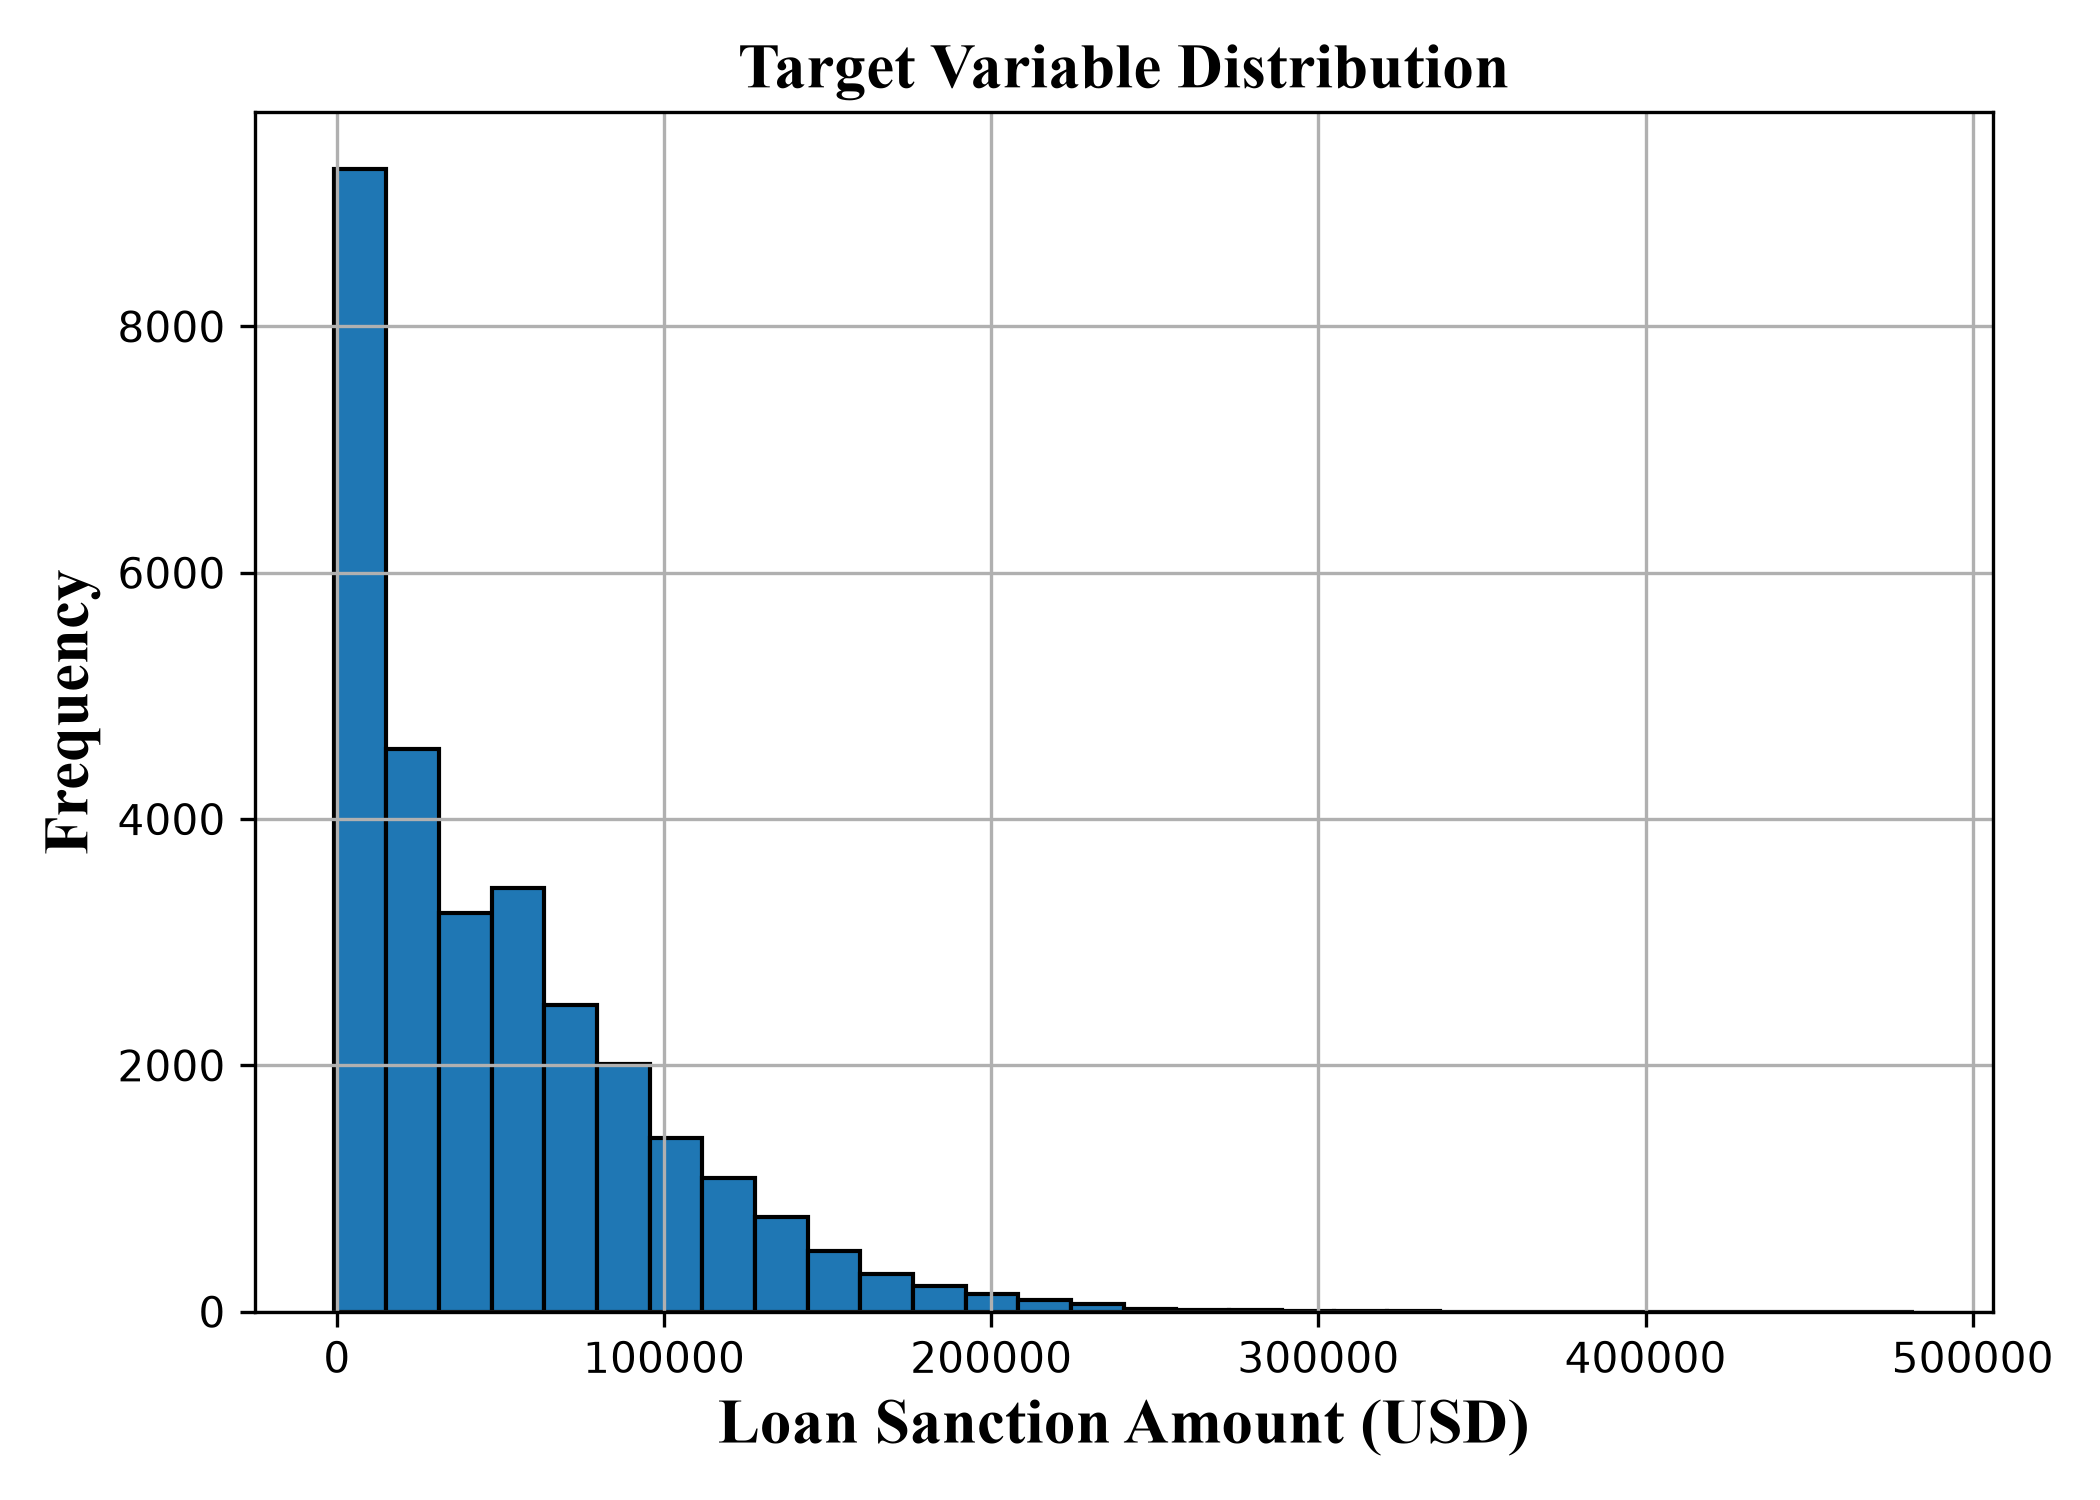
\includegraphics[width=0.7\linewidth]{target_distribution.png}
\caption{Distribution of Loan Sanction Amount}
\end{figure}

\textbf{Inference:}

The target variable is right-skewed, with most loan sanction amounts concentrated in the lower-to-mid range (roughly \$0--\$75{,}000) and a long tail extending toward higher amounts approaching \$480{,}000. A visible spike near zero corresponds to applications that were rejected or sanctioned a nominal amount. This skew suggests that outlier customers with very high sanctioned amounts may disproportionately influence ordinary least-squares coefficients, which motivates the use of regularized models alongside plain Linear Regression to control the resulting variance.

\subsection{Feature vs Target Relationships}

\begin{figure}[H]
\centering
\includegraphics[width=0.7\linewidth]{age_vs_target.png}
\caption{Age vs Loan Sanction Amount}
\end{figure}

\textbf{Inference:}

Age shows a very weak relationship with the target variable (correlation $= 0.0081$), with sanctioned amounts spread broadly and almost uniformly across all age groups from 18 to 65. This indicates that age alone is not a meaningful predictor of loan sanction amount and mainly serves to fine-tune predictions in combination with other features rather than driving them independently.

\begin{figure}[H]
\centering
\includegraphics[width=0.7\linewidth]{income_vs_target.png}
\caption{Income vs Loan Sanction Amount}
\end{figure}

\textbf{Inference:}

Income shows a surprisingly weak linear relationship with the target, with a correlation of only 0.038. This is counter-intuitive given that income should logically drive loan capacity, and is best explained by the extreme outliers in the income column (max $\approx \$1.78$ million against a median of $\approx \$2222$), which compress the visible linear trend and reduce the Pearson correlation. This suggests income may be more predictive after outlier capping or log-transformation, which was not applied in this iteration of the pipeline but is noted as a possible improvement.

\begin{figure}[H]
\centering
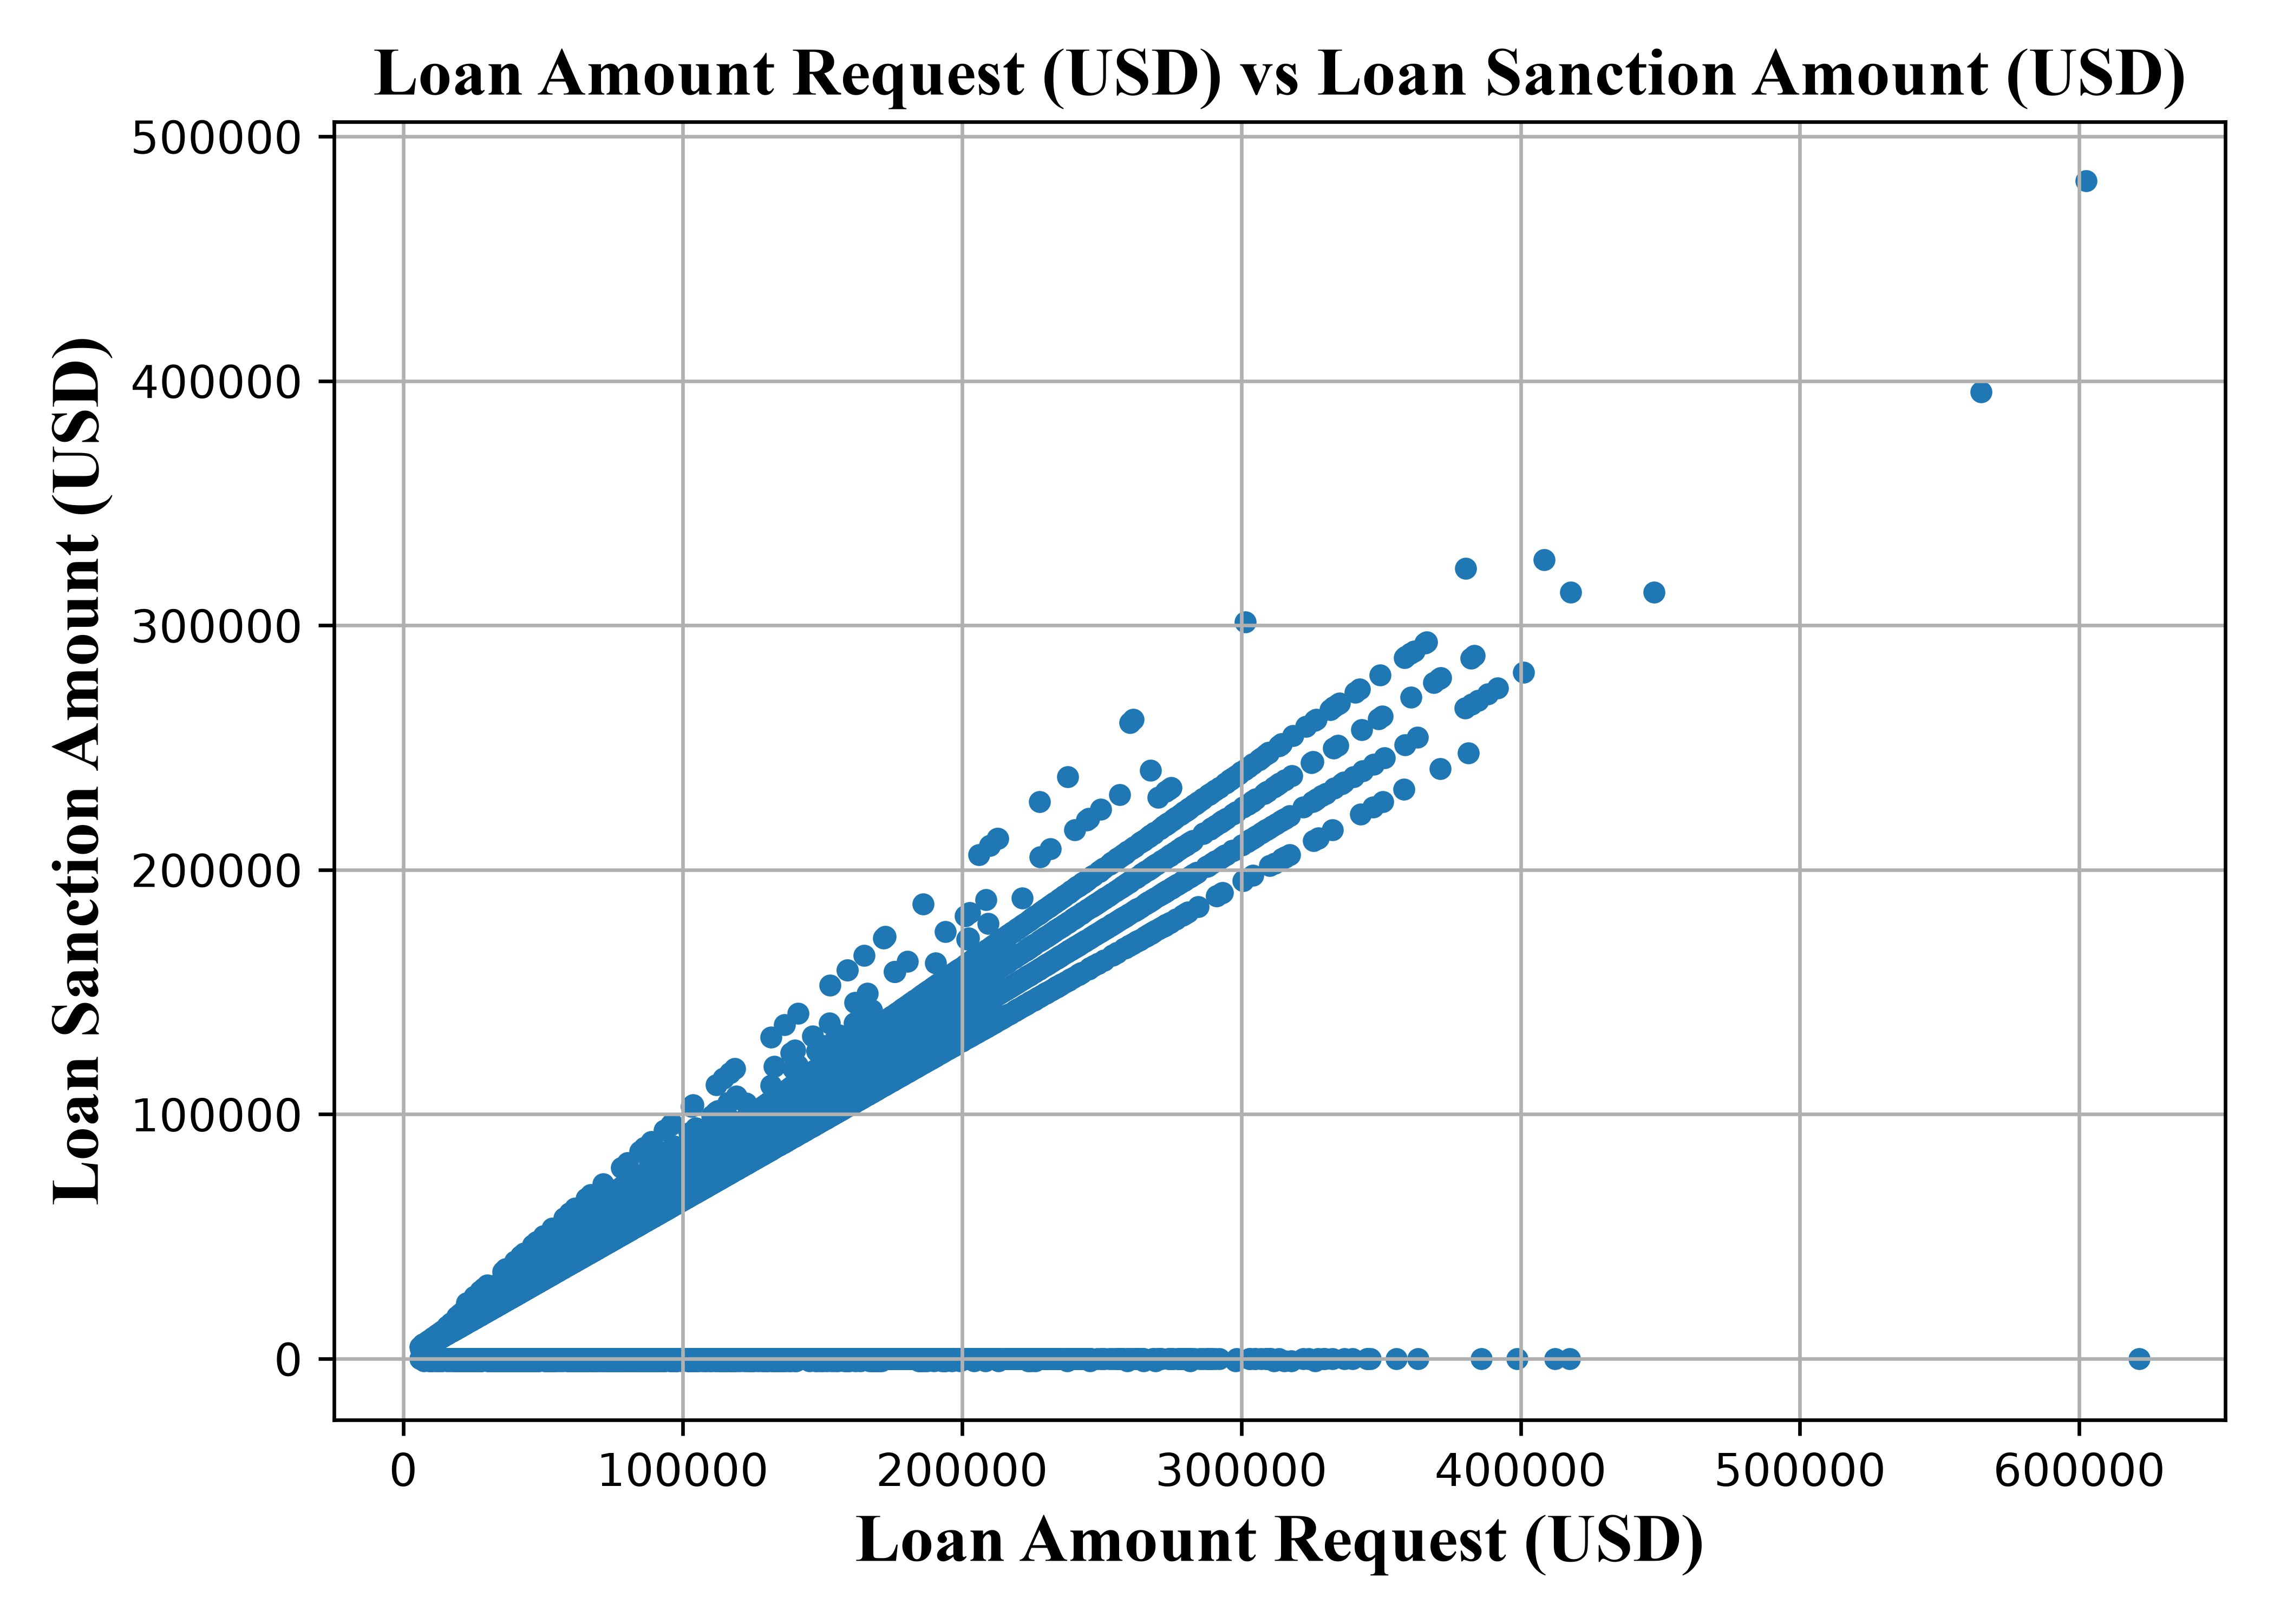
\includegraphics[width=0.7\linewidth]{loan_amount_request_vs_target.png}
\caption{Loan Amount Request vs Loan Sanction Amount}
\end{figure}

\textbf{Inference:}

Loan Amount Request shows the strongest positive correlation with the target variable (0.726), confirming that the amount requested by a customer is the single most influential factor in determining the sanctioned amount. The scatter plot shows a clear near-linear band, consistent with lenders typically sanctioning a fraction of the requested amount rather than an unrelated value.

\begin{figure}[H]
\centering
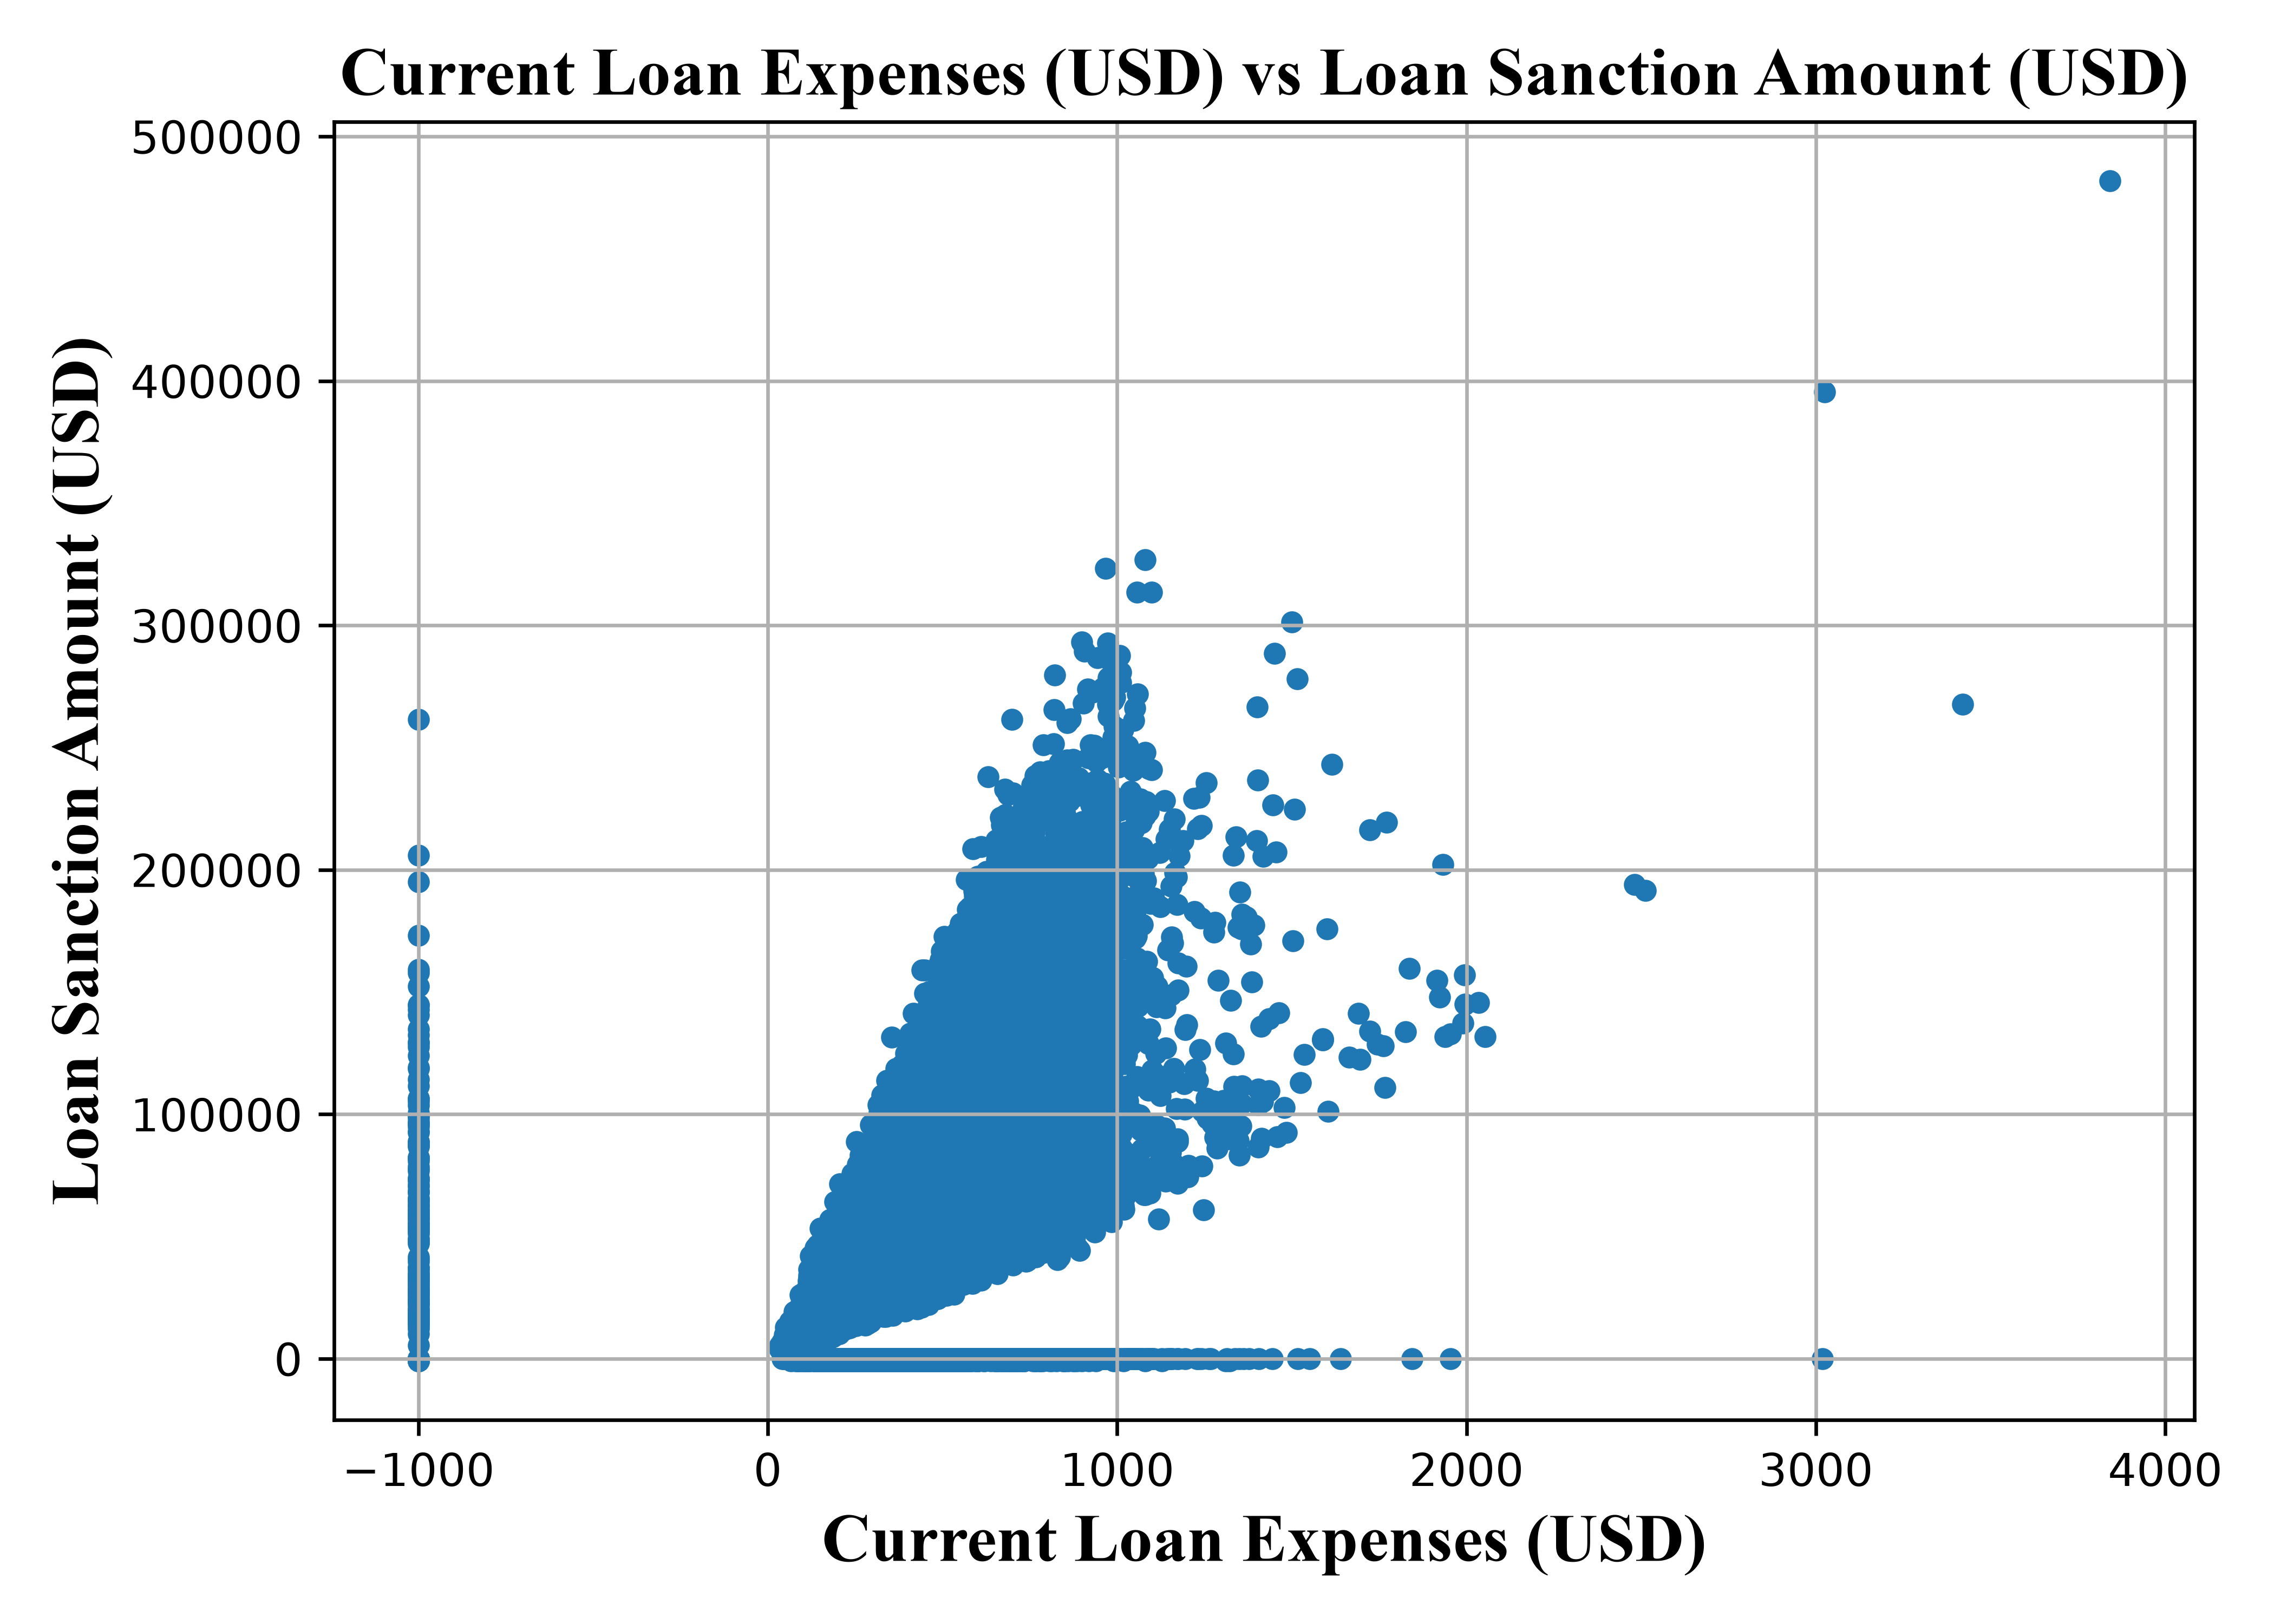
\includegraphics[width=0.7\linewidth]{current_loan_expenses_vs_target.png}
\caption{Current Loan Expenses vs Loan Sanction Amount}
\end{figure}

\textbf{Inference:}

Current Loan Expenses shows a moderate positive correlation (0.485) with the target, suggesting that customers with higher ongoing loan expenses tend to be sanctioned higher loan amounts, likely reflecting their overall financial profile and existing creditworthiness rather than expense burden being penalized.

\begin{figure}[H]
\centering
\includegraphics[width=0.7\linewidth]{dependents_vs_target.png}
\caption{Dependents vs Loan Sanction Amount}
\end{figure}

\textbf{Inference:}

The number of dependents shows a very weak relationship with the target variable (correlation $= 0.009$), indicating that family size has minimal direct influence on the sanctioned loan amount compared to financial and property-related features. This is consistent with lending decisions being driven more by repayment capacity and collateral than household composition.

\subsection{Correlation Analysis}

The correlation matrix was generated using numerical features to identify relationships between variables.

\begin{figure}[H]
\centering
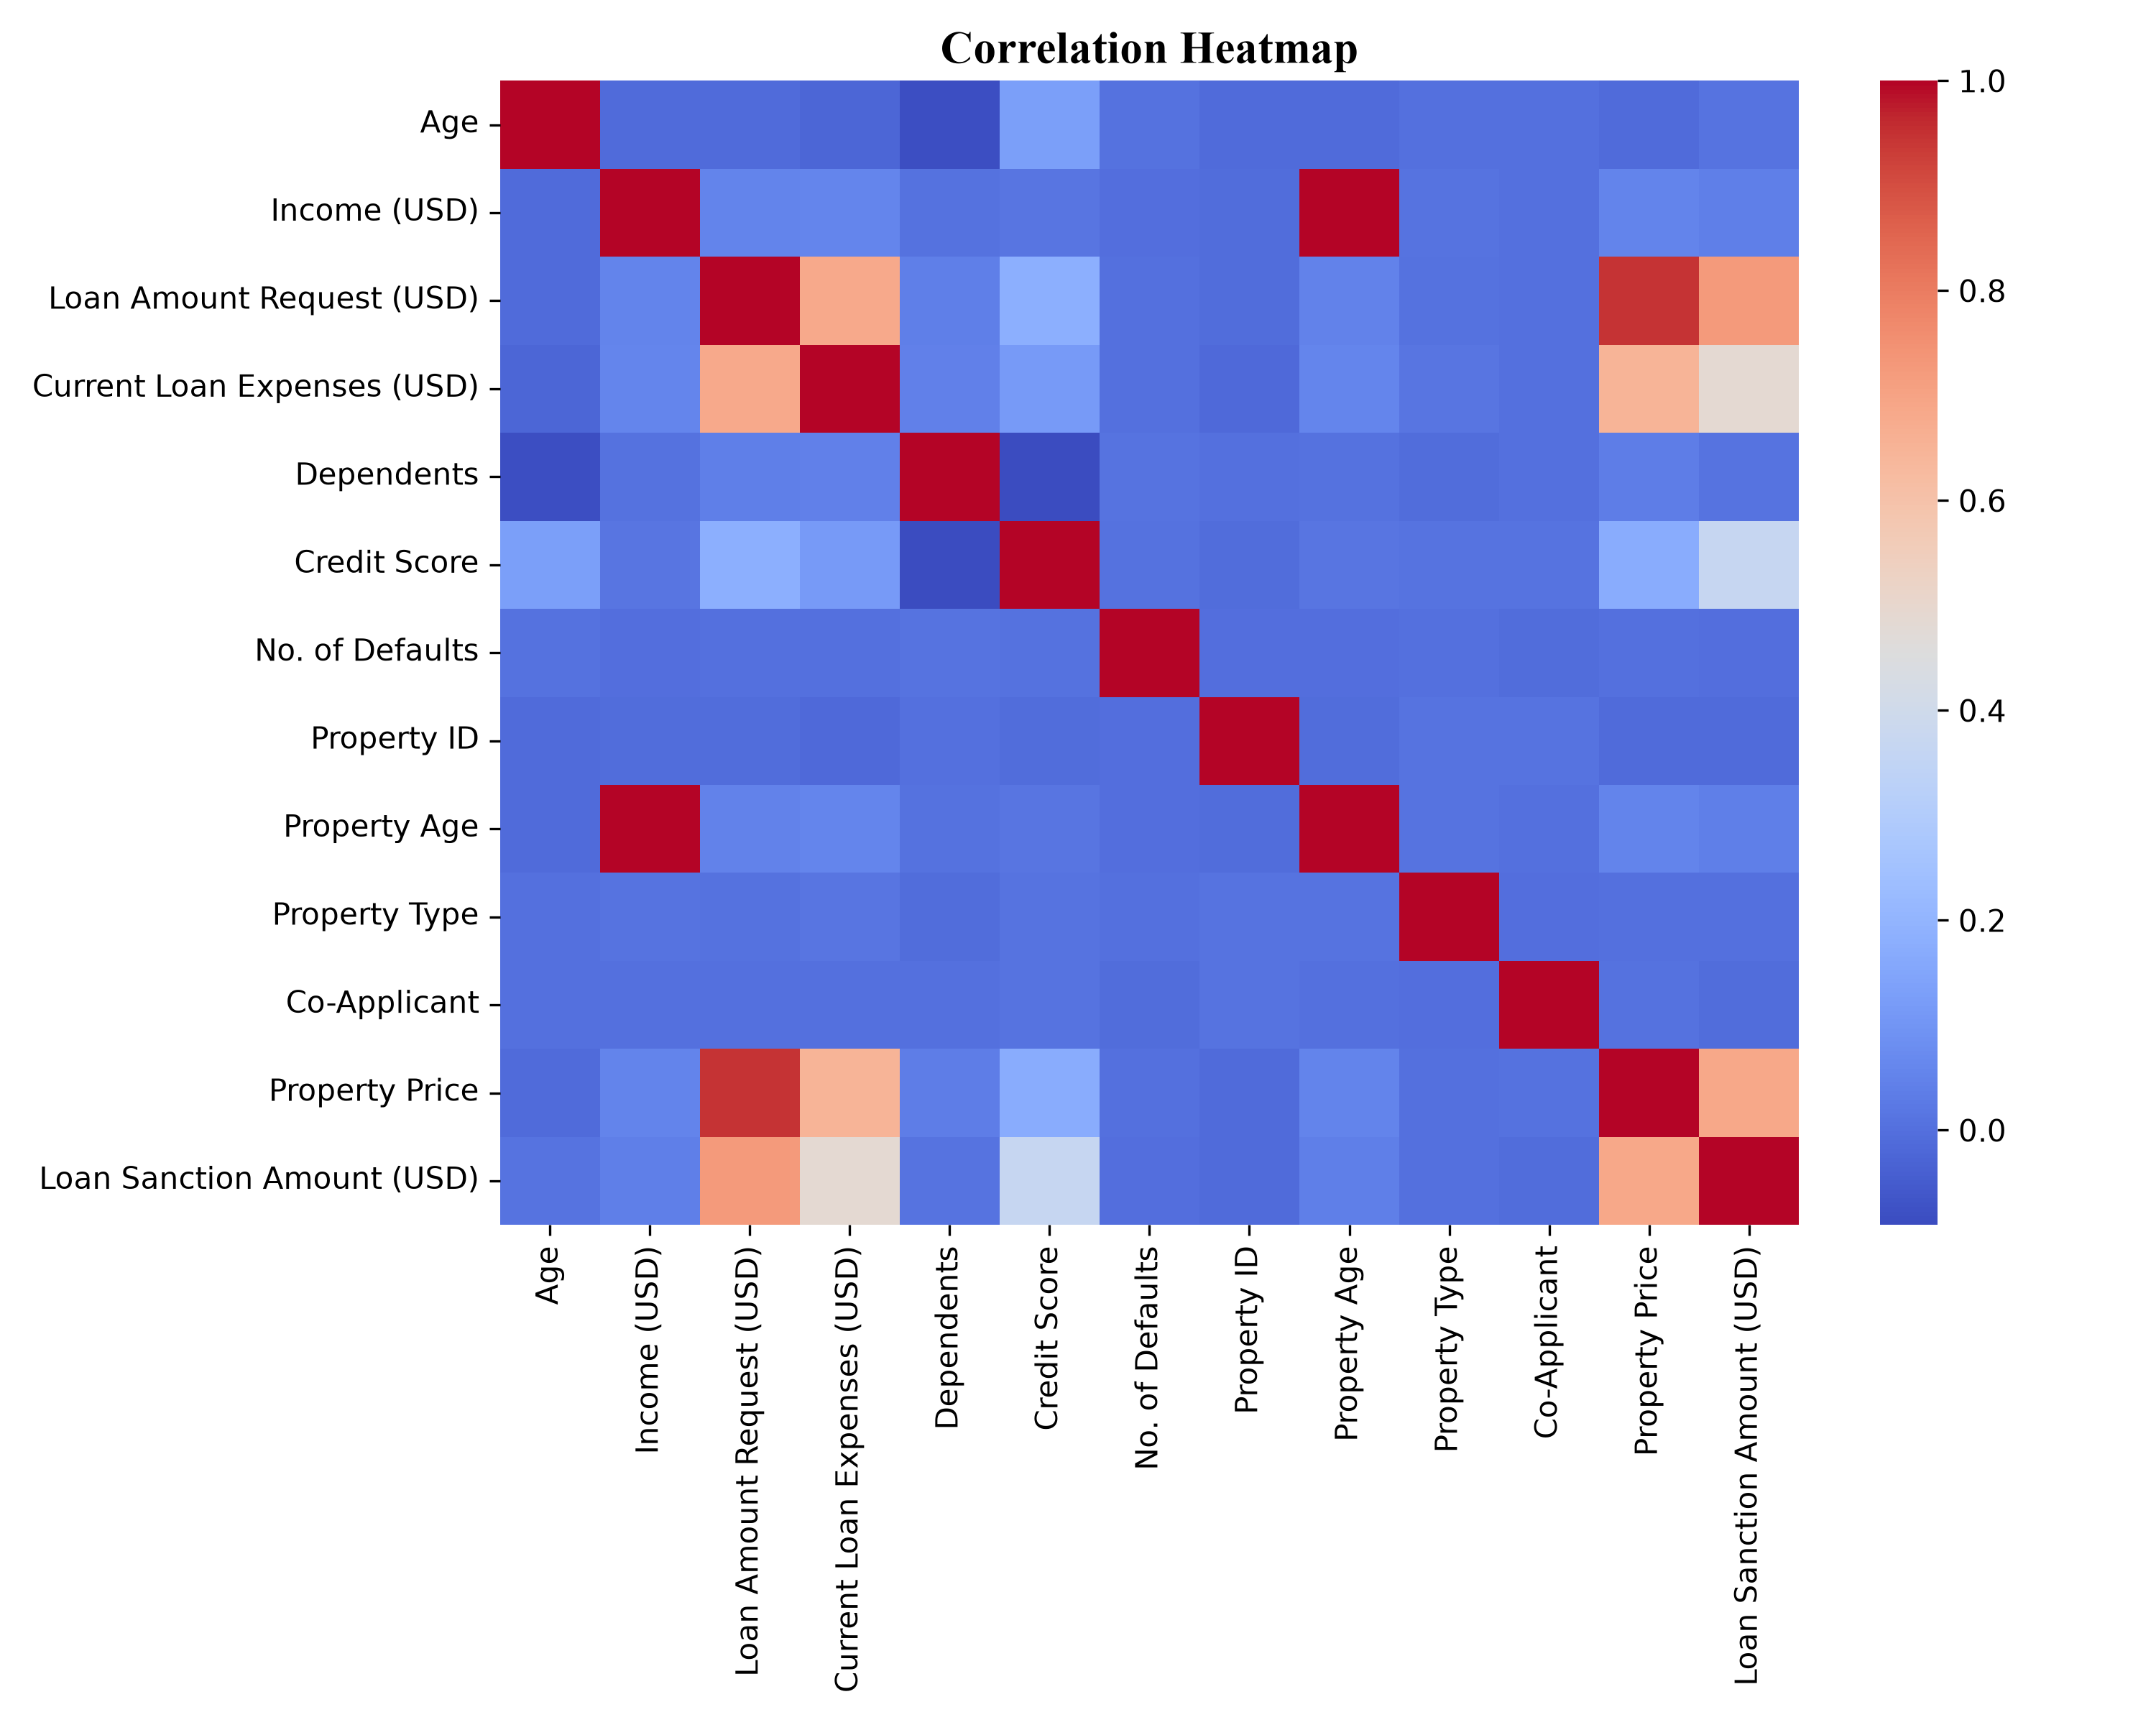
\includegraphics[width=0.7\linewidth]{correlation_heatmap.png}
\caption{Correlation Heatmap of Numerical Features}
\end{figure}

\begin{table}[H]
\centering
\begin{tabular}{lc}
\toprule
Feature & Correlation with Target \\
\midrule
Loan Amount Request (USD) & 0.7264 \\
Property Price & 0.6871 \\
Current Loan Expenses (USD) & 0.4851 \\
Credit Score & 0.3694 \\
Income (USD) & 0.0381 \\
Property Age & 0.0378 \\
Dependents & 0.0091 \\
Age & 0.0081 \\
Property Type & 0.0020 \\
No. of Defaults & -0.0043 \\
Co-Applicant & -0.0069 \\
Property ID & -0.0098 \\
\bottomrule
\end{tabular}
\caption{Correlation of All Numerical Features with Loan Sanction Amount}
\end{table}

\textbf{Inference:}

Loan Amount Request and Property Price have by far the strongest influence on the loan sanction amount, together capturing most of the explainable linear variance. Credit Score also contributes significantly, since customers with better credit history generally receive higher sanctioned amounts relative to their request. Attributes such as Age, Dependents, Property Type, and No. of Defaults show near-zero linear correlation with the target, implying that a large share of the 53-dimensional feature space (after one-hot encoding) contributes little unique linear signal -- which is precisely the setting in which L1-based feature selection (Lasso) is expected to be beneficial.

\section{Data Preprocessing}

Data preprocessing was performed to convert the raw dataset into a suitable format for regression algorithms, using a single \texttt{scikit-learn} \texttt{ColumnTransformer} pipeline to ensure that the exact same transformations (fit on training data only) are applied consistently to the test set.

\subsection{Removal of Unnecessary Attributes}

The following columns were removed because they are unique identifiers or free-text fields that do not contribute meaningful predictive information: \textbf{Customer ID}, \textbf{Name}, and \textbf{Property ID}.

\subsection{Handling Missing Symbols}

Before imputation, several placeholder symbols representing missing data were first replaced with \texttt{NaN} so that they would not be silently treated as valid numeric values:

\begin{itemize}
\item \texttt{?}
\item \texttt{-999}
\item Empty strings
\item \texttt{NA}
\end{itemize}

\subsection{Missing Value Handling}

For numerical features, missing values were replaced using \textbf{mean imputation}, chosen to reduce the effect of outliers relative to more extreme substitution strategies while keeping the pipeline simple and reproducible.

For categorical features, missing values were replaced using the \textbf{most frequent category} (mode imputation), which preserves the existing category distribution as closely as possible.

\subsection{Categorical Feature Encoding}

Categorical variables were converted into numerical form using \textbf{One-Hot Encoding}, which creates separate binary indicator features for each category while gracefully handling unknown categories that might appear only in the test set (via \texttt{handle\_unknown='ignore'}).

\subsection{Feature Scaling}

Numerical features were standardized using \texttt{StandardScaler}:

\[
X_{scaled} = \frac{X-\mu}{\sigma}
\]

where $\mu$ represents the mean of the feature and $\sigma$ represents the standard deviation. Feature scaling improves convergence for regularized models and ensures that features with larger numeric ranges (e.g. Income, Property Price) do not dominate the regularization penalty relative to smaller-scale features (e.g. Dependents, Age).

\subsection{Train-Test Split}

The processed dataset was divided into training and testing sets using an 80/20 split.

\begin{table}[H]
\centering
\begin{tabular}{lc}
\toprule
Dataset & Samples \\
\midrule
Training Data & 23457 \\
Testing Data & 5865 \\
\bottomrule
\end{tabular}
\caption{Train-Test Dataset Distribution}
\end{table}

The preprocessing pipeline generated:
\[
X_{train} = (23457, 53), \qquad X_{test} = (5865, 53)
\]

After preprocessing, the final feature space contained 53 numerical features (expanded from the original set via one-hot encoding of categorical attributes), which were used for regression model training.

\section{Implementation Details}

The implementation was modularized using reusable functions organized into dedicated source modules (\texttt{preprocessing.py}, \texttt{regression.py}, \texttt{validation.py}, \texttt{metrics.py}, \texttt{timing.py}, \texttt{visualization.py}, \texttt{eda.py}):

\begin{itemize}
\item \texttt{perform\_regression\_eda()} -- runs the complete exploratory analysis and saves the consolidated summary figure.
\item \texttt{preprocess\_data()} -- builds and applies the preprocessing pipeline (imputation, encoding, scaling, splitting).
\item \texttt{train\_regression()} -- trains a specified regression algorithm with given hyperparameters.
\item \texttt{tune\_regression\_model()} -- performs GridSearchCV-based hyperparameter optimization.
\item \texttt{compare\_regression\_models()} -- computes MAE, MSE, RMSE, and R$^2$ on the test set for all models.
\item \texttt{compare\_cross\_validation()} -- performs 5-fold cross-validation and reports training vs. validation error.
\item \texttt{get\_coefficients()} -- extracts fitted coefficients for interpretability analysis.
\item \texttt{compare\_training\_prediction\_time()} -- benchmarks training and prediction runtime for each model.
\end{itemize}

This modular design allows each stage of the pipeline (EDA, preprocessing, training, tuning, evaluation, visualization) to be reused across other experiments in the same laboratory course with minimal changes.

\section{Machine Learning Algorithm}

Regression algorithms are supervised learning techniques used to predict continuous numerical values. In this experiment, four regression models are implemented and compared: Linear Regression, Ridge Regression, Lasso Regression, and Elastic Net Regression.

\subsection{Linear Regression}

Linear Regression models the relationship between input features and the target variable by fitting a linear equation:
\[
y = \beta_0 + \beta_1 x_1 + \beta_2 x_2 + \dots + \beta_n x_n
\]
where $y$ is the predicted loan sanction amount, $x_1, x_2, \dots, x_n$ are the input features, $\beta_0$ is the intercept, and $\beta_1, \dots, \beta_n$ are the feature coefficients.

The objective of Linear Regression is to minimize the residual sum of squares:
\[
RSS = \sum_{i=1}^{n}(y_i - \hat{y}_i)^2
\]
where $y_i$ is the actual value and $\hat{y}_i$ is the predicted value, solved in closed form via the normal equations (or an equivalent least-squares solver).

\textbf{Advantages:} Simple and easy to interpret; computationally efficient; works well when relationships are approximately linear.

\textbf{Limitations:} Sensitive to outliers; performs poorly with highly correlated (multicollinear) features; cannot capture complex nonlinear relationships.

\subsection{Ridge Regression}

Ridge Regression is a regularized version of Linear Regression that reduces model complexity by adding an L2 penalty term:
\[
Loss = \sum_{i=1}^{n}(y_i-\hat{y}_i)^2 + \lambda\sum_{j=1}^{m}\beta_j^2
\]
where $\lambda$ is the regularization parameter and $\beta_j$ are the model coefficients. Ridge regression shrinks large coefficient values toward zero (but not exactly to zero) and improves model generalization, particularly when features are correlated.

\textbf{Advantages:} Handles multicollinearity effectively; reduces overfitting; retains all features in the final model.

\textbf{Limitations:} Does not perform feature selection; requires careful selection of the regularization strength $\lambda$.

\subsection{Lasso Regression}

Lasso Regression applies L1 regularization by adding the absolute values of coefficients as a penalty term:
\[
Loss = \sum_{i=1}^{n}(y_i-\hat{y}_i)^2 + \lambda\sum_{j=1}^{m}|\beta_j|
\]
The L1 penalty forces some coefficients to become exactly zero, which performs automatic feature selection -- effectively removing features that do not meaningfully improve predictive accuracy.

\textbf{Advantages:} Performs feature selection; produces simpler, more interpretable models; reduces overfitting.

\textbf{Limitations:} May arbitrarily remove one of several highly correlated important features; sensitive to the choice of regularization parameter.

\subsection{Elastic Net Regression}

Elastic Net combines both L1 and L2 regularization techniques:
\[
Loss = \sum_{i=1}^{n}(y_i-\hat{y}_i)^2 + \lambda\left(\alpha\sum|\beta_j| + (1-\alpha)\sum\beta_j^2\right)
\]
where $\alpha$ controls the contribution of L1 regularization and $(1-\alpha)$ controls the contribution of L2 regularization. Elastic Net provides the benefits of both Ridge and Lasso regression, and is particularly useful when there are groups of correlated features, since it tends to select or shrink them together rather than arbitrarily picking one.

\textbf{Advantages:} Handles correlated features better than Lasso alone; performs feature selection; reduces overfitting.

\textbf{Limitations:} Requires tuning of multiple hyperparameters ($\alpha$ and $l1\_ratio$); more computationally expensive than Ridge or Lasso individually.

\section{Experimental Setup}

\begin{table}[H]
\centering
\begin{tabular}{ll}
\toprule
Parameter & Details \\
\midrule
Programming Language & Python \\
Machine Learning Library & Scikit-Learn \\
Data Processing Library & Pandas, NumPy \\
Visualization Library & Matplotlib \\
Development Environment & Jupyter Notebook \\
Python Version & Python 3.x (Anaconda Environment) \\
Operating System & Linux (Anaconda Environment) \\
Dataset Size & 30000 samples \\
Processor & Intel-based system \\
\bottomrule
\end{tabular}
\caption{Experimental Environment}
\end{table}

\subsection*{Initial (Untuned) Model Configuration}

\begin{table}[H]
\centering
\begin{tabular}{lll}
\toprule
Model & Regularization & Parameters \\
\midrule
Linear Regression & None & Default \\
Ridge & L2 & $\alpha = 1$ \\
Lasso & L1 & $\alpha = 0.1$ \\
Elastic Net & L1 + L2 & $\alpha = 0.1,\ l1\_ratio = 0.5$ \\
\bottomrule
\end{tabular}
\caption{Initial Regression Model Parameters (Before Tuning)}
\end{table}

\section{Hyperparameter Selection}

GridSearchCV was used to find optimal regularization parameters, using a 5-fold cross-validation strategy with R$^2$ score as the evaluation metric.

\begin{table}[H]
\centering
\begin{tabular}{lll}
\toprule
Model & Parameter Search Space & Best Parameter \\
\midrule
Ridge & $\alpha \in \{0.01,0.1,1,10,100\}$ & $\alpha = 100$ \\
Lasso & $\alpha \in \{0.001,0.01,0.1,1,10\}$ & $\alpha = 10$ \\
Elastic Net & $\alpha \in \{0.01,0.1,1,10\}$ & $\alpha = 0.1$ \\
 & $l1\_ratio \in \{0.2,0.5,0.8\}$ & $l1\_ratio = 0.8$ \\
\bottomrule
\end{tabular}
\caption{Hyperparameter Optimization Results}
\end{table}

\begin{table}[H]
\centering
\begin{tabular}{lc}
\toprule
Model & Best CV R$^2$ Score \\
\midrule
Ridge & 0.5923 \\
Lasso & 0.5921 \\
Elastic Net & 0.5939 \\
\bottomrule
\end{tabular}
\caption{Grid Search Cross-Validation Performance}
\end{table}

\textbf{Inference:} Ridge selected the largest permissible $\alpha$ (100) from its search space, suggesting that strong L2 shrinkage was beneficial given the moderate multicollinearity among engineered one-hot features. Lasso settled on $\alpha = 10$, a relatively strong penalty, consistent with many of the 53 features carrying little independent signal. Elastic Net's chosen $l1\_ratio = 0.8$ indicates that the optimal blend leaned heavily toward L1-style sparsity while still retaining a small L2 component for stability.

\section{Performance Evaluation Metrics}

The trained regression models were evaluated using the following standard regression metrics.

\subsection*{Mean Absolute Error (MAE)}
\[
MAE = \frac{1}{n}\sum_{i=1}^{n}|y_i - \hat{y}_i|
\]
Lower MAE indicates better average prediction accuracy in the original units of the target (USD).

\subsection*{Mean Squared Error (MSE)}
\[
MSE = \frac{1}{n}\sum_{i=1}^{n}(y_i - \hat{y}_i)^2
\]
MSE penalizes larger errors more heavily than MAE due to the squaring operation, making it more sensitive to outlier predictions.

\subsection*{Root Mean Squared Error (RMSE)}
\[
RMSE = \sqrt{MSE}
\]
RMSE expresses error in the same unit as the target variable (USD), making it more directly interpretable than MSE.

\subsection*{R$^2$ Score}
\[
R^2 = 1 - \frac{\sum(y_i-\hat{y}_i)^2}{\sum(y_i-\bar{y})^2}
\]
R$^2$ represents the proportion of variance in the target explained by the model; higher values indicate better fit, with $1.0$ representing a perfect fit and $0.0$ representing performance equivalent to predicting the mean.

\section{Results}

\subsection{Test Set Performance}

\begin{table}[H]
\centering
\begin{tabular}{lrrrr}
\toprule
Model & MAE & MSE & RMSE & R$^2$ Score \\
\midrule
Linear Regression & 20754.89 & 8.95$\times10^{8}$ & 29917.03 & 0.6021 \\
Ridge Regression & 20768.96 & 8.95$\times10^{8}$ & 29921.56 & 0.6020 \\
Lasso Regression & 20737.56 & 8.94$\times10^{8}$ & 29903.95 & 0.6024 \\
Elastic Net & 20871.54 & 9.00$\times10^{8}$ & 30000.72 & 0.5999 \\
\bottomrule
\end{tabular}
\caption{Regression Model Performance on Test Data}
\end{table}

\textbf{Inference:} All regression models achieved similar performance because the dataset contains strong linear relationships between important features and the target variable. Lasso Regression obtained the highest R$^2$ score (0.6024) and the lowest RMSE (29903.95) among the tested models, narrowly outperforming Linear and Ridge Regression. Elastic Net trailed the other three by a small margin, likely because its selected $\alpha$ and $l1\_ratio$ trade a marginal amount of test accuracy for improved coefficient stability across resampling.

\subsection{Cross-Validation Performance}

Five-fold cross-validation was performed to verify model stability across different training subsets.

\begin{table}[H]
\centering
\begin{tabular}{lrrrr}
\toprule
Model & MAE & RMSE & R$^2$ Score & Validation Error (MSE) \\
\midrule
Linear Regression & 21103.77 & 30788.17 & 0.5947 & 9.48$\times10^{8}$ \\
Ridge Regression & 21108.41 & 30760.81 & 0.5954 & 9.46$\times10^{8}$ \\
Lasso Regression & 21081.06 & 30750.04 & 0.5957 & 9.45$\times10^{8}$ \\
Elastic Net & 21175.97 & 30777.02 & 0.5950 & 9.47$\times10^{8}$ \\
\bottomrule
\end{tabular}
\caption{5-Fold Cross-Validation Results}
\end{table}

\textbf{Inference:} The cross-validation results are consistent with the held-out test performance, both in ranking and in absolute magnitude, which strongly suggests the test split is representative and the models are not overfit to a particular partition of the data. Lasso Regression achieved the highest average validation R$^2$ score (0.5957), showing the best generalization ability among the four models. Ridge and Elastic Net also performed consistently, indicating that regularization helped reduce model variance without materially harming bias.

\section{Result Visualization}

\subsection{Actual vs Predicted Plot}

\begin{figure}[H]
\centering
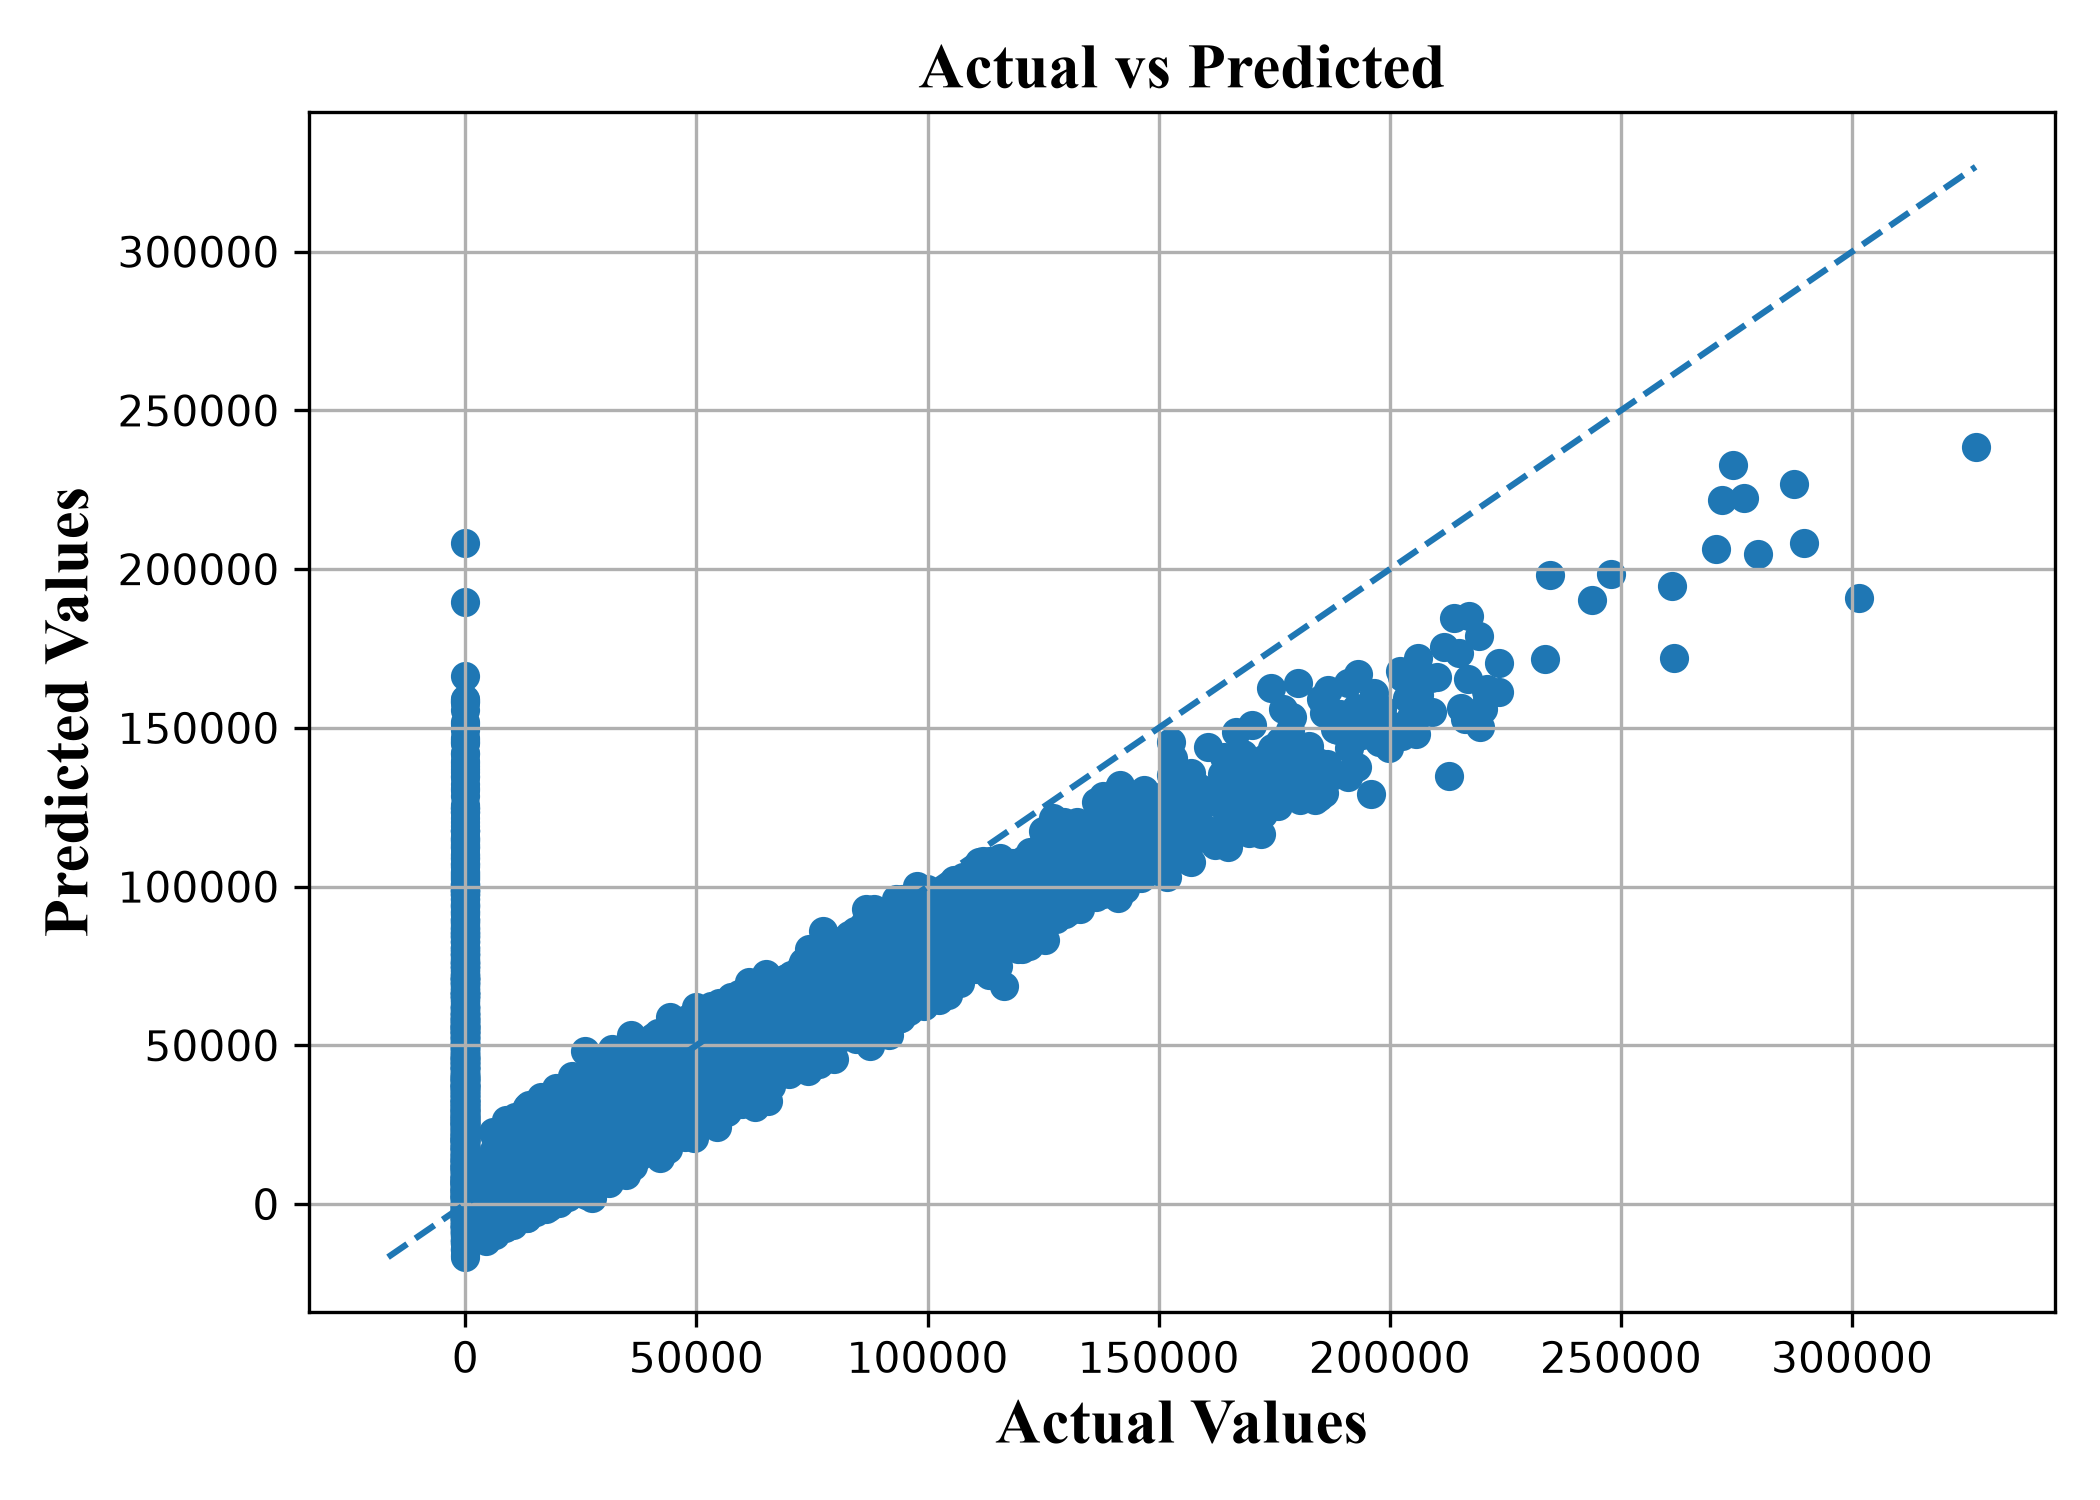
\includegraphics[width=0.7\linewidth]{model_actual_vs_predicted.png}
\caption{Actual vs Predicted Loan Sanction Amount (Elastic Net)}
\end{figure}

\textbf{Inference:} The actual versus predicted plot shows the relationship between predicted loan sanction amounts and true values. Points closer to the diagonal line indicate accurate predictions. The model captures the overall trend of loan sanction values reasonably well in the low-to-mid range, but visibly under-predicts for customers with very high actual sanction amounts -- consistent with the right-skewed target distribution observed during EDA, where extreme values are comparatively rare and harder for a linear model to fit precisely.

\subsection{Residual Analysis}

\begin{figure}[H]
\centering
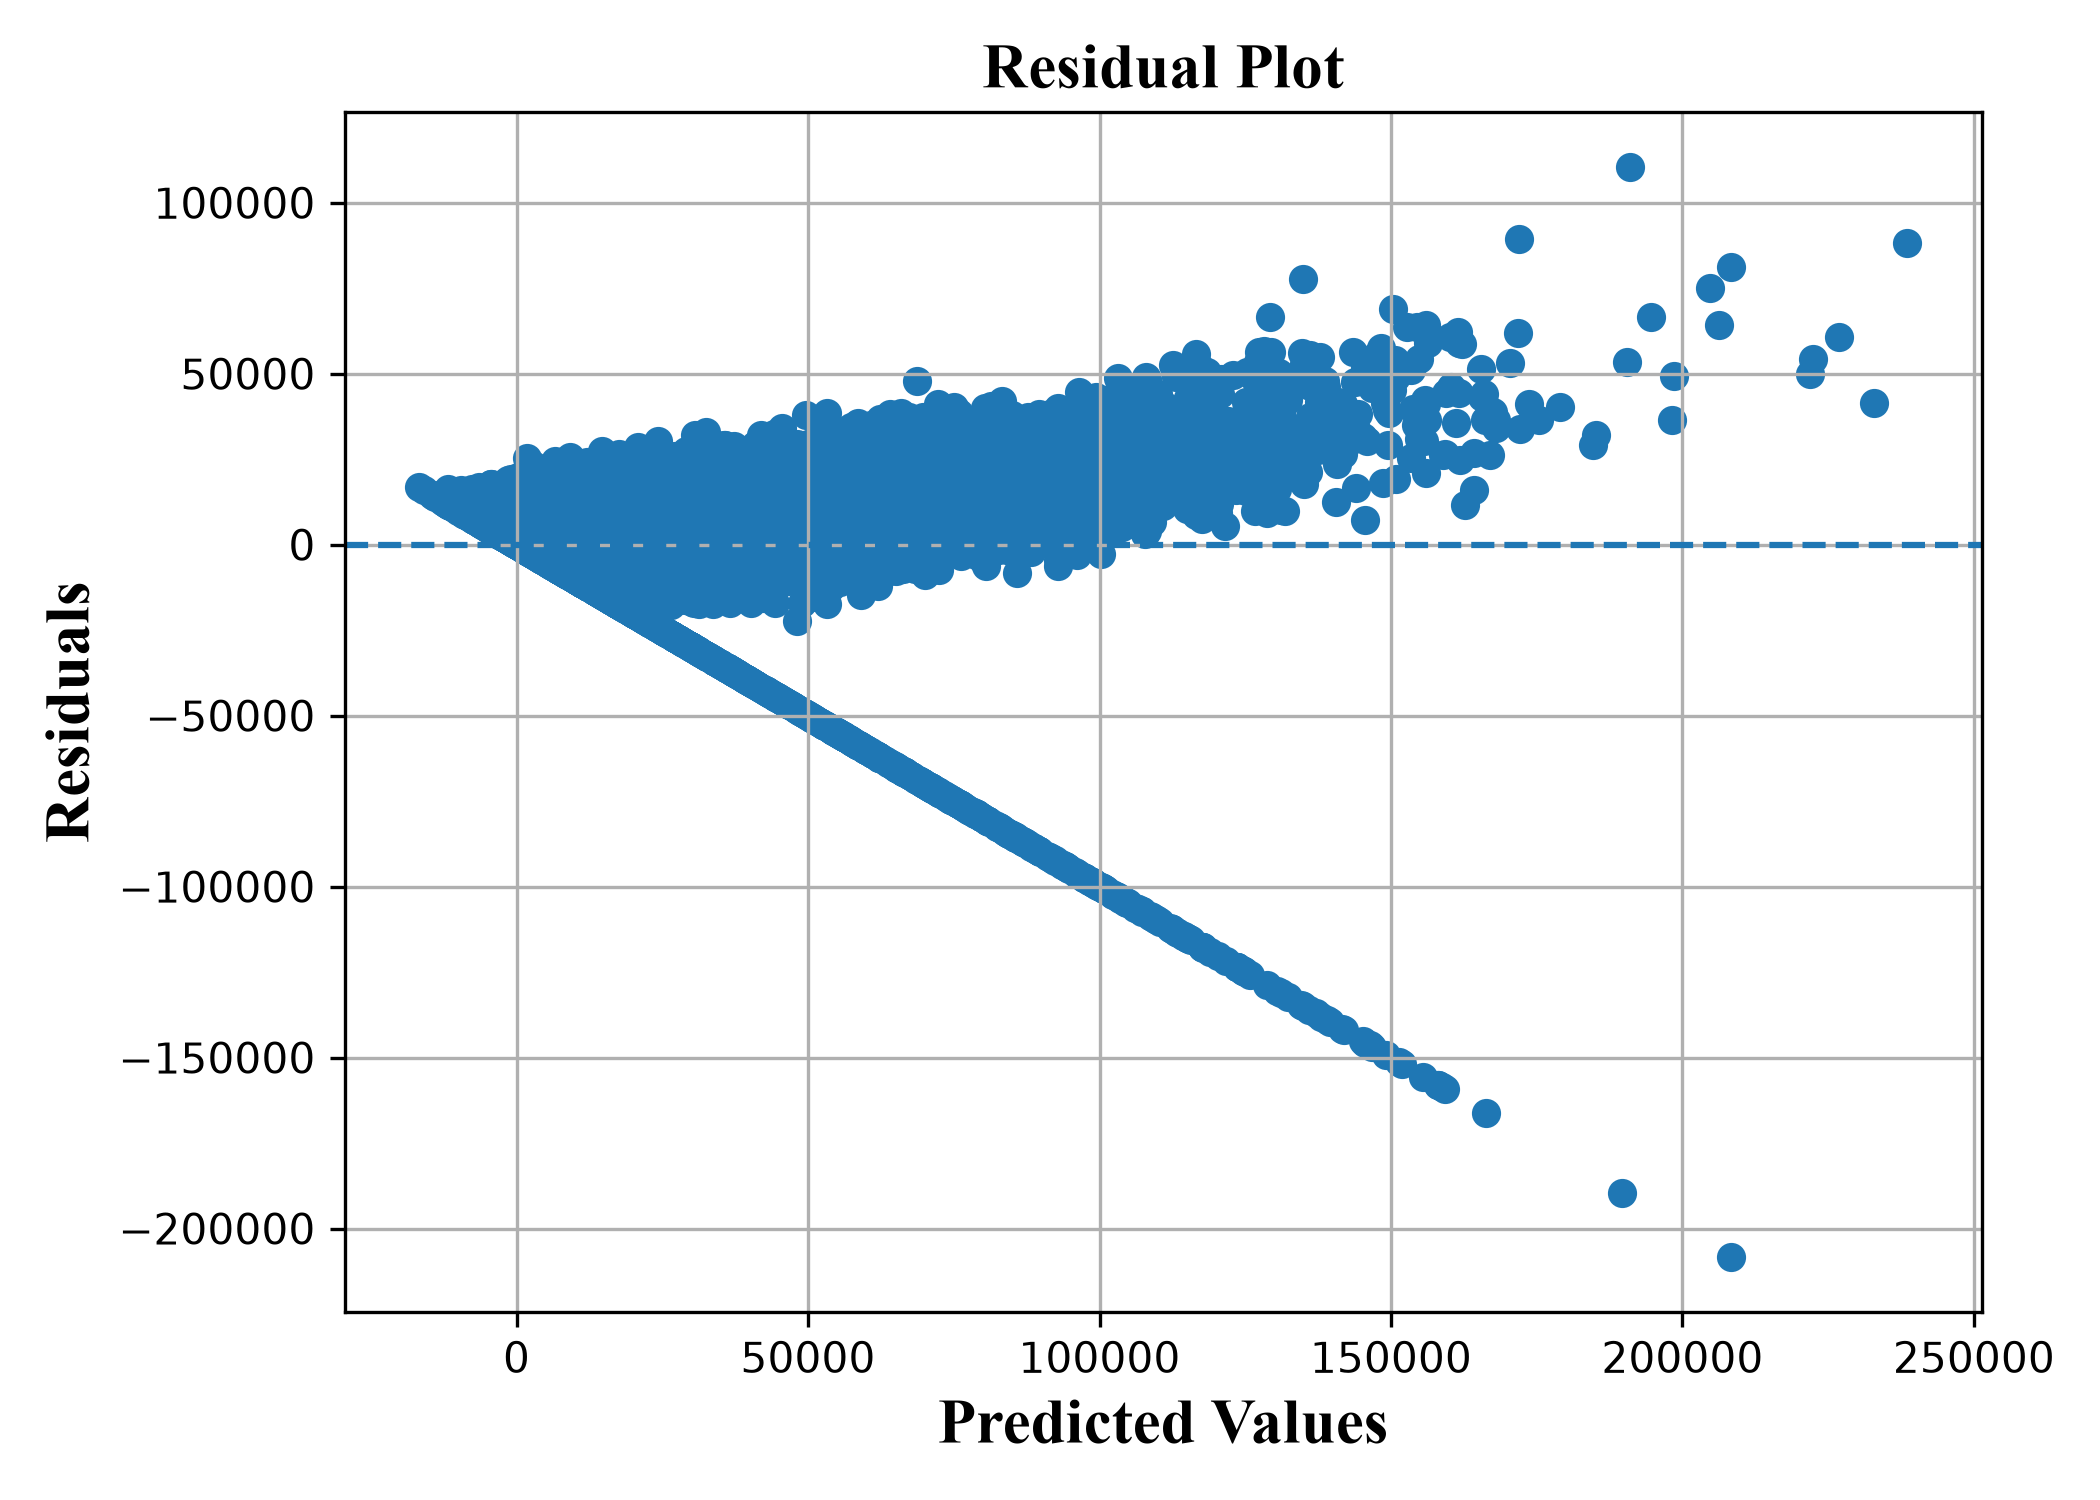
\includegraphics[width=0.7\linewidth]{model_residual_plot.png}
\caption{Residual Distribution Plot}
\end{figure}

\textbf{Inference:} The residual plot is used to analyze prediction errors. Residuals are distributed roughly around zero across the bulk of predictions, indicating that the model does not show significant systematic bias for typical loan amounts. Some larger residuals (outliers) are present at the extremes, which may be attributable to unusually high income or property values in the dataset that are not fully captured by the linear relationship, reinforcing the earlier observation that a small subset of records disproportionately drives error.

\section{Model Coefficient Analysis}

Regression coefficients were analyzed to understand the contribution of different features and how each regularization scheme reshapes them.

\begin{table}[H]
\centering
\begin{tabular}{lrrrr}
\toprule
Feature & Linear & Ridge & Lasso & Elastic Net \\
\midrule
Age & -589.09 & -558.67 & -553.76 & -540.02 \\
Income (USD) & 31491.86 & 615.81 & 27.08 & 144.58 \\
Loan Amount Request (USD) & 34691.84 & 33207.53 & 34499.90 & 29206.40 \\
Current Loan Expenses (USD) & -956.91 & -771.42 & -910.78 & -223.10 \\
Dependents & -55.12 & -54.69 & -42.03 & -52.65 \\
\bottomrule
\end{tabular}
\caption{Sample of Regression Coefficients Across Models (First 5 Features)}
\end{table}

\begin{figure}[H]
\centering
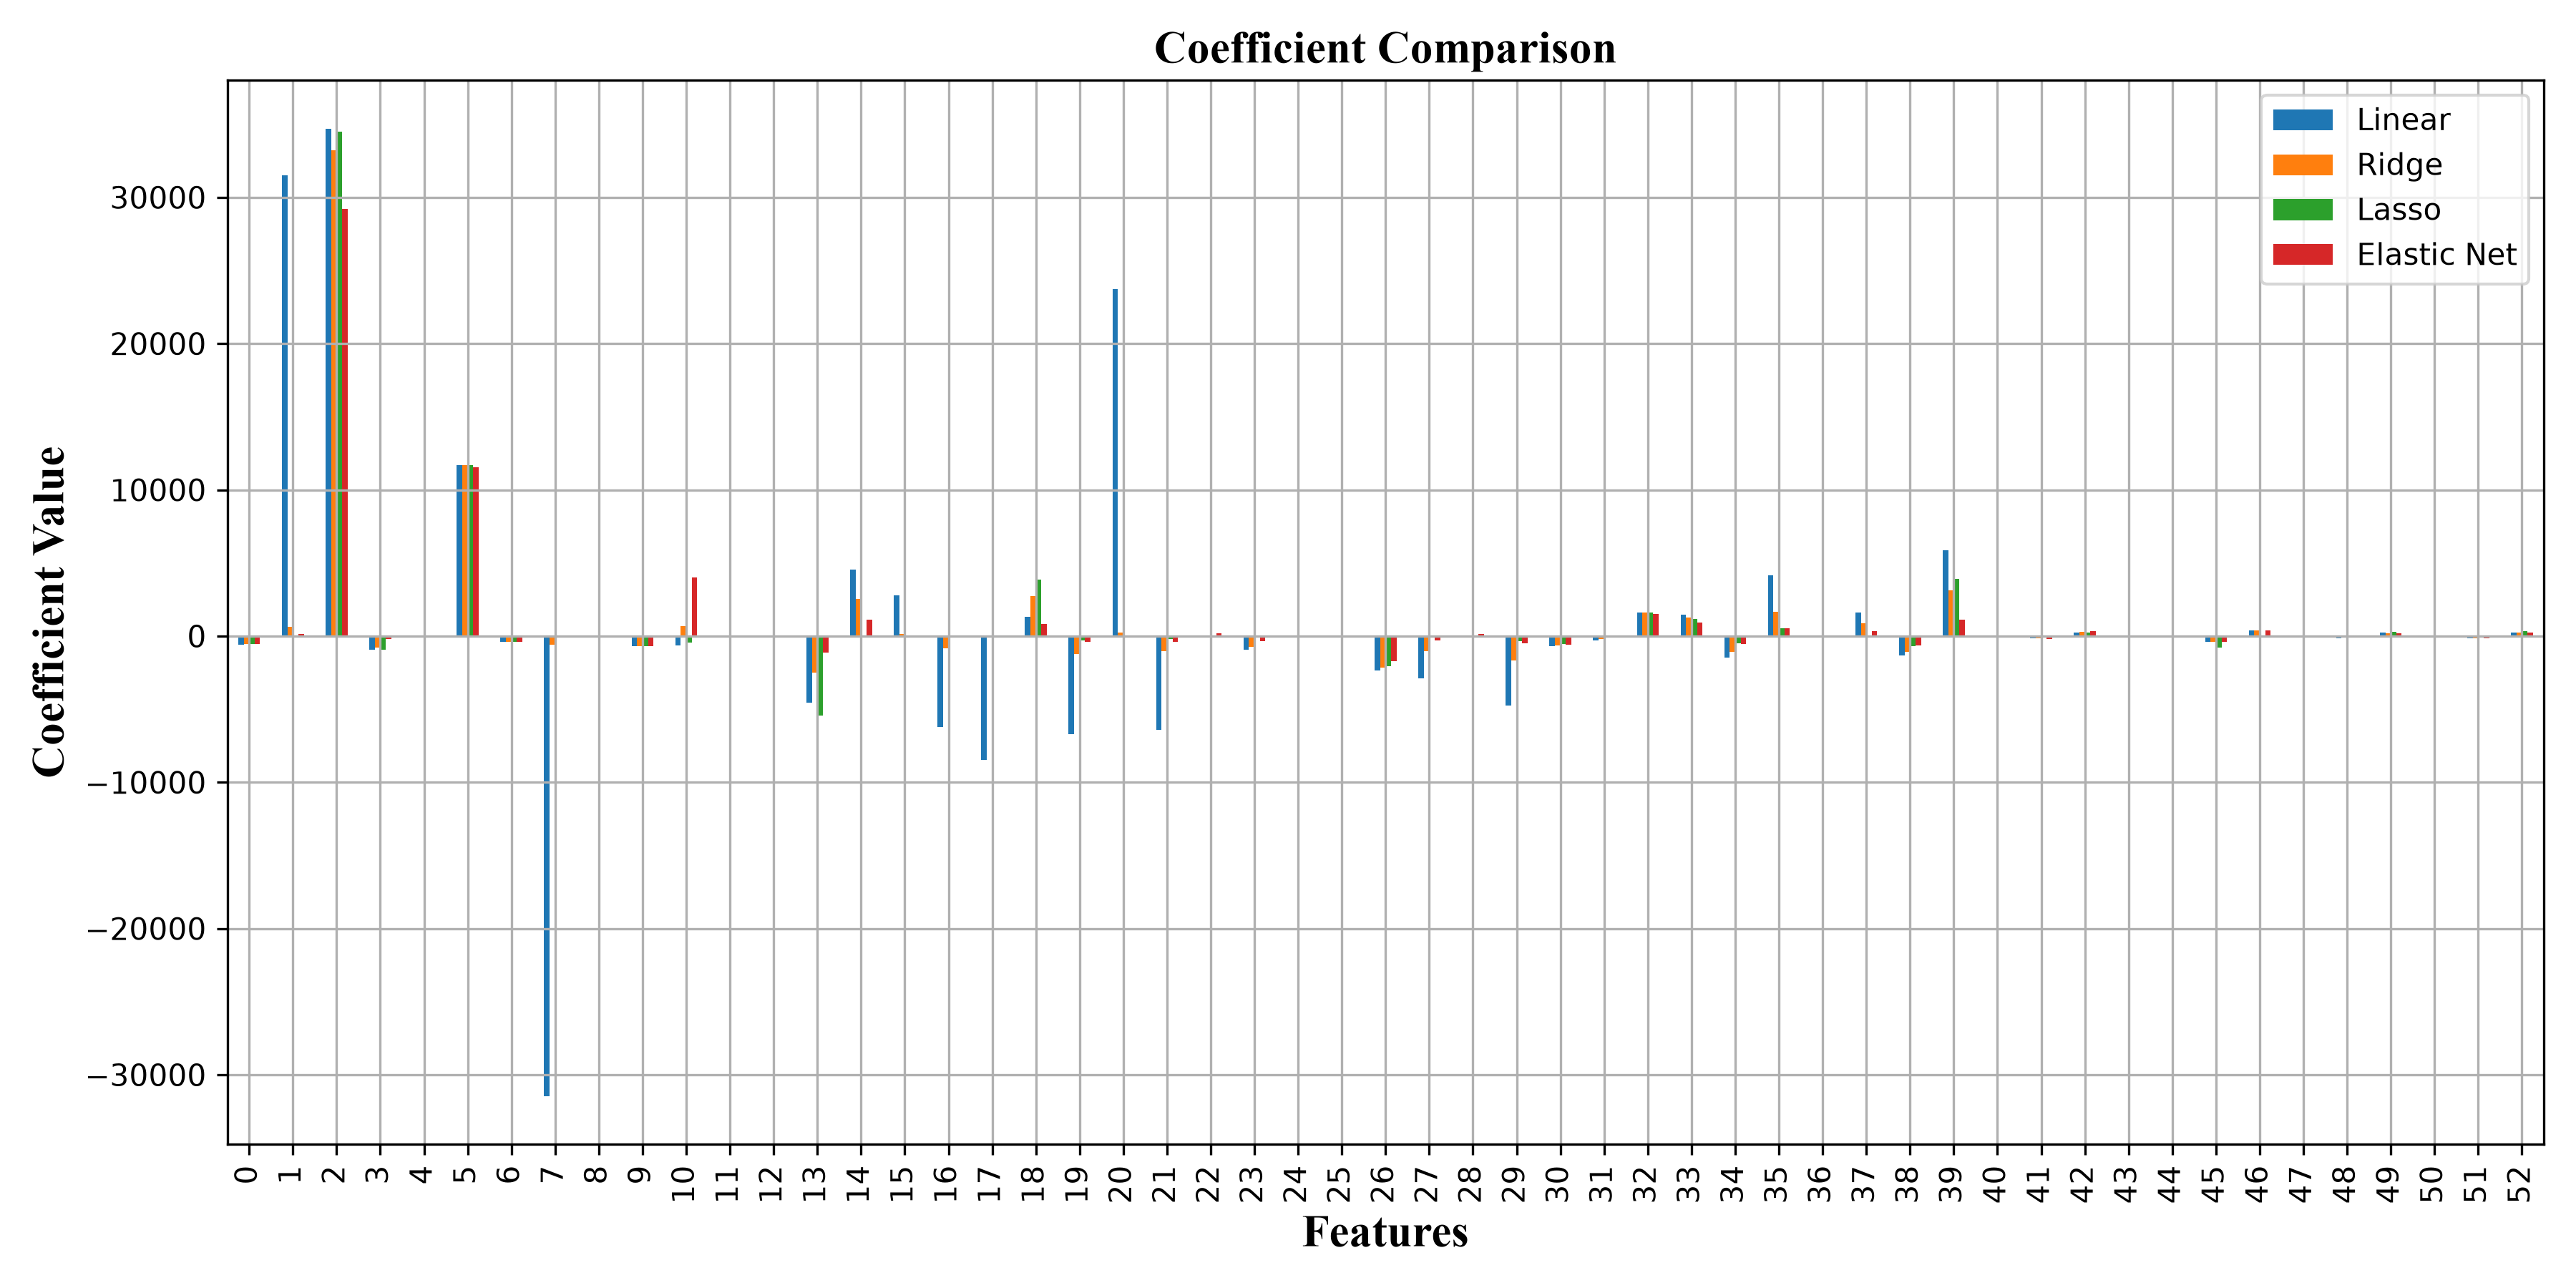
\includegraphics[width=0.85\linewidth]{coefficient_comparison.png}
\caption{Coefficient Comparison Between Regression Models}
\end{figure}

\textbf{Inference:} The coefficient comparison shows the dramatic effect of regularization on feature weights. Linear Regression produces the largest and most volatile coefficients -- most notably for Income (USD), where the unregularized coefficient (31491.86) is over 1000$\times$ larger than the Lasso coefficient (27.08). This is a clear symptom of the outlier-driven instability identified during EDA: because a handful of extreme income values are present, unregularized least squares overreacts to them, while Ridge, Lasso, and Elastic Net all pull this coefficient sharply toward zero. By contrast, the Loan Amount Request coefficient remains large and stable across all four models (29206--34691), confirming it as a robust, model-agnostic predictor. Lasso is visibly the most aggressive at shrinking less informative coefficients (e.g. Income, Dependents) toward zero, consistent with its role as an implicit feature-selection mechanism.

\subsection*{Training vs Validation Error Curve}

\begin{figure}[H]
\centering
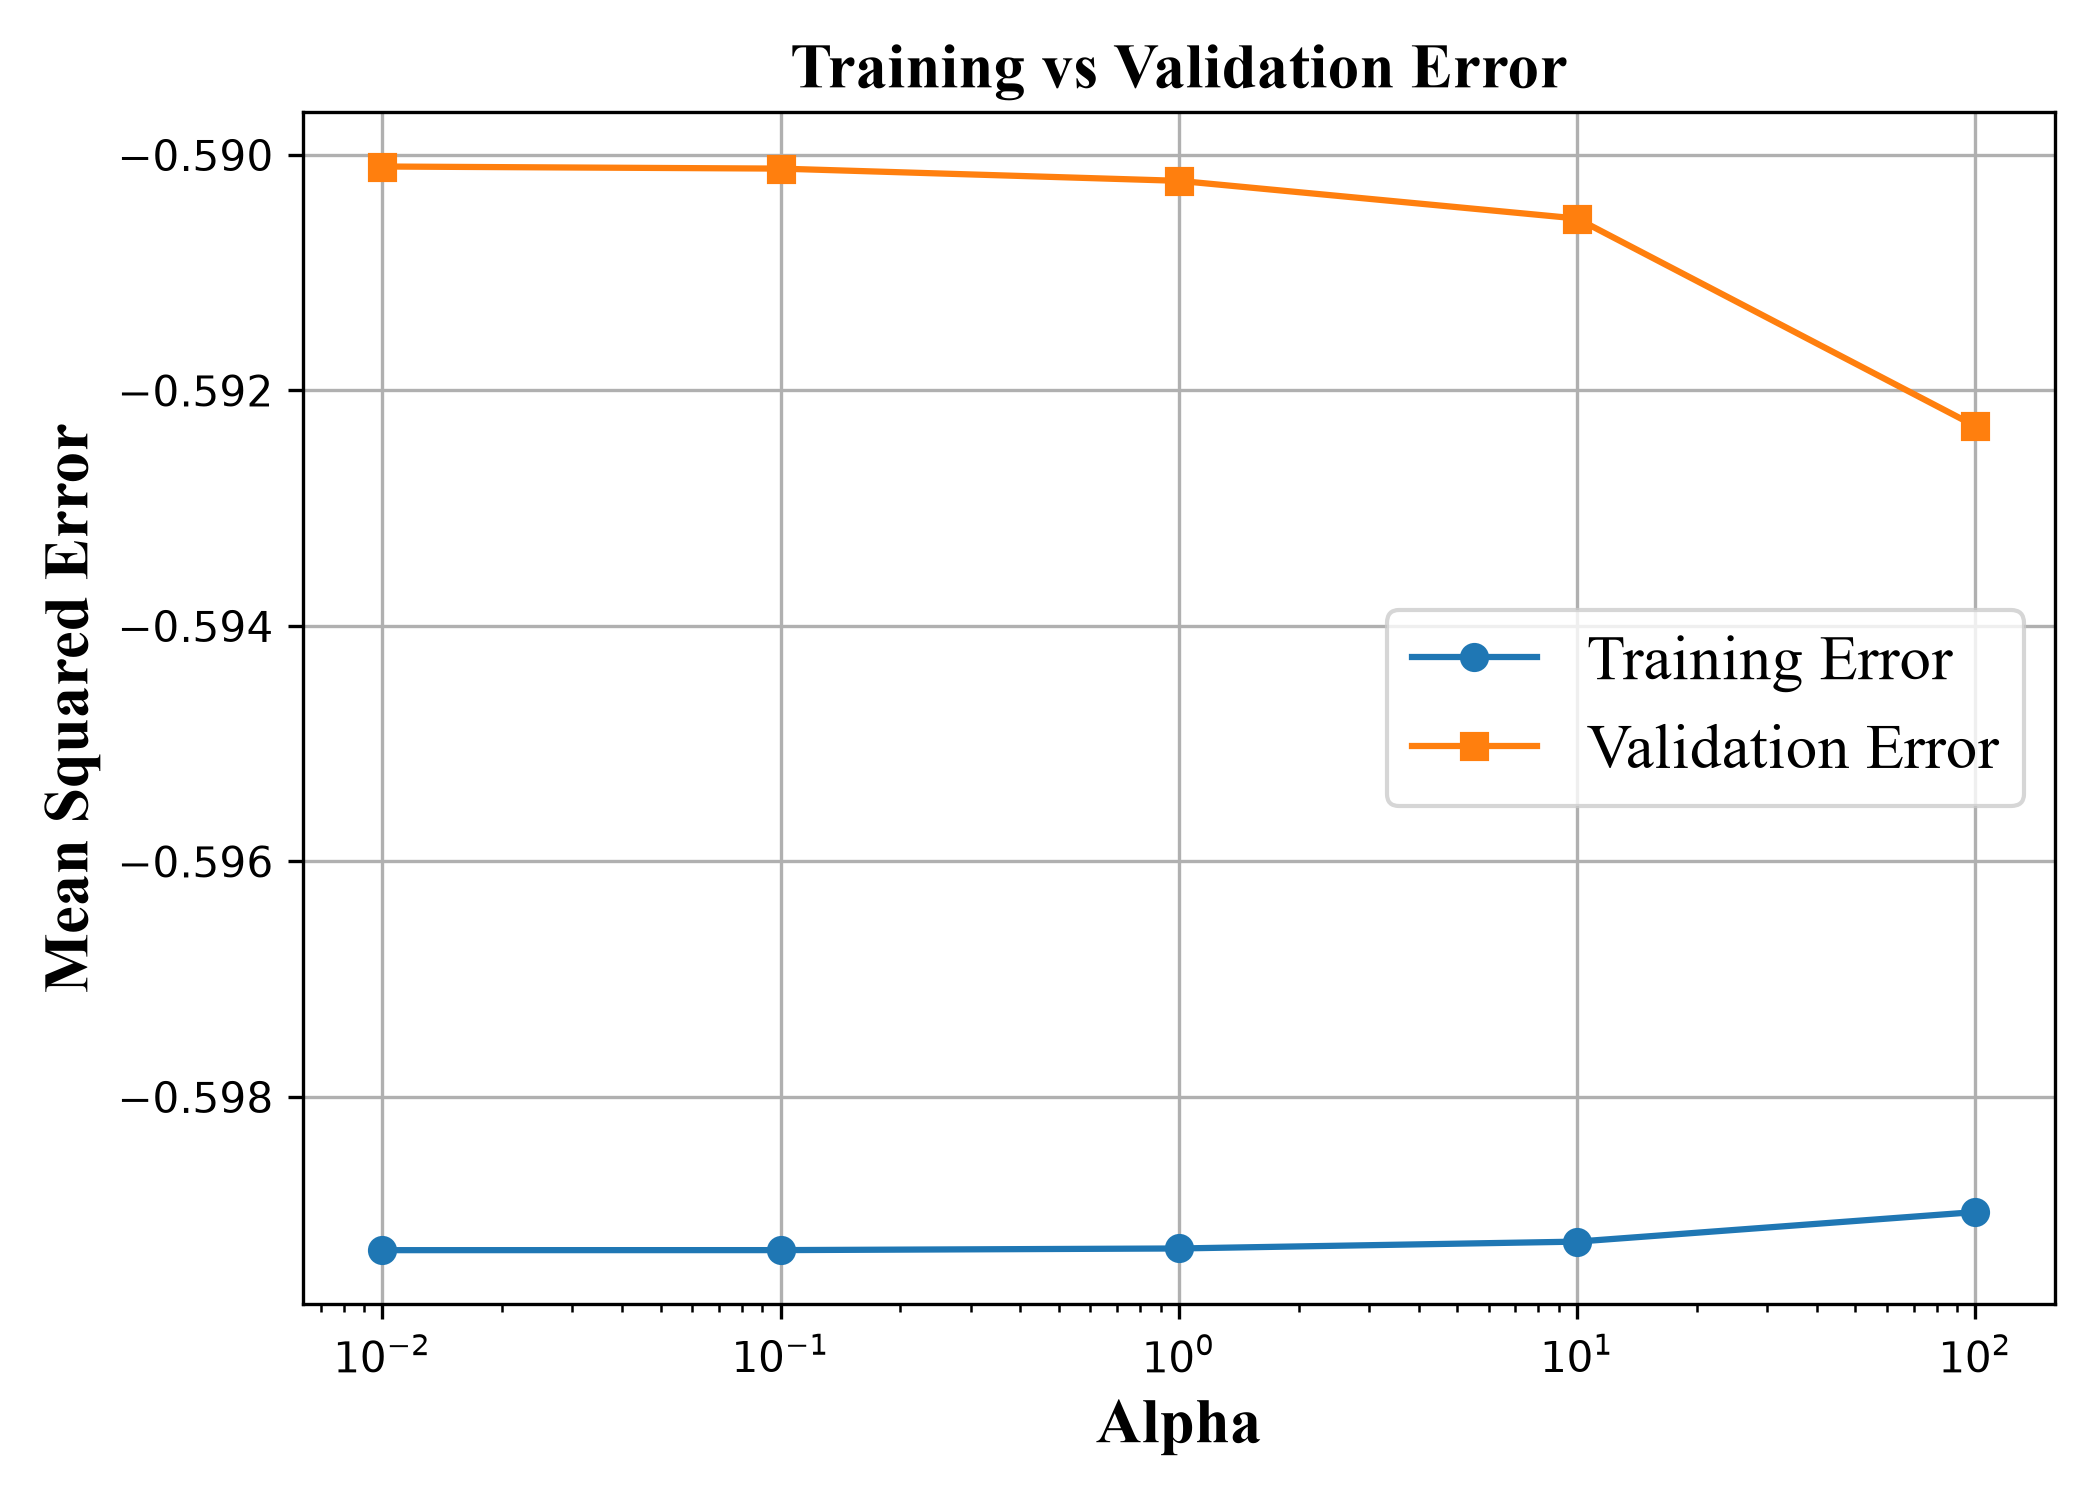
\includegraphics[width=0.7\linewidth]{training_validation_error.png}
\caption{Training Error vs Validation Error (Ridge, across $\alpha$ values)}
\end{figure}

\textbf{Inference:} As the regularization strength $\alpha$ increases, training error rises slightly (since the model is prevented from fitting the training data as tightly), while validation error initially decreases and then stabilizes. This is the classic signature of regularization successfully trading a small amount of bias for a larger reduction in variance, up to a point beyond which further increases in $\alpha$ would begin to underfit.

\section{Execution Time Analysis}

\begin{table}[H]
\centering
\begin{tabular}{lrr}
\toprule
Model & Training Time (s) & Prediction Time (s) \\
\midrule
Linear Regression & 0.0528 & 0.0007 \\
Ridge Regression & 0.0186 & 0.0017 \\
Lasso Regression & 0.4259 & 0.0011 \\
Elastic Net & 0.8752 & 0.0008 \\
\bottomrule
\end{tabular}
\caption{Training and Prediction Time Comparison}
\end{table}

\begin{figure}[H]
\centering
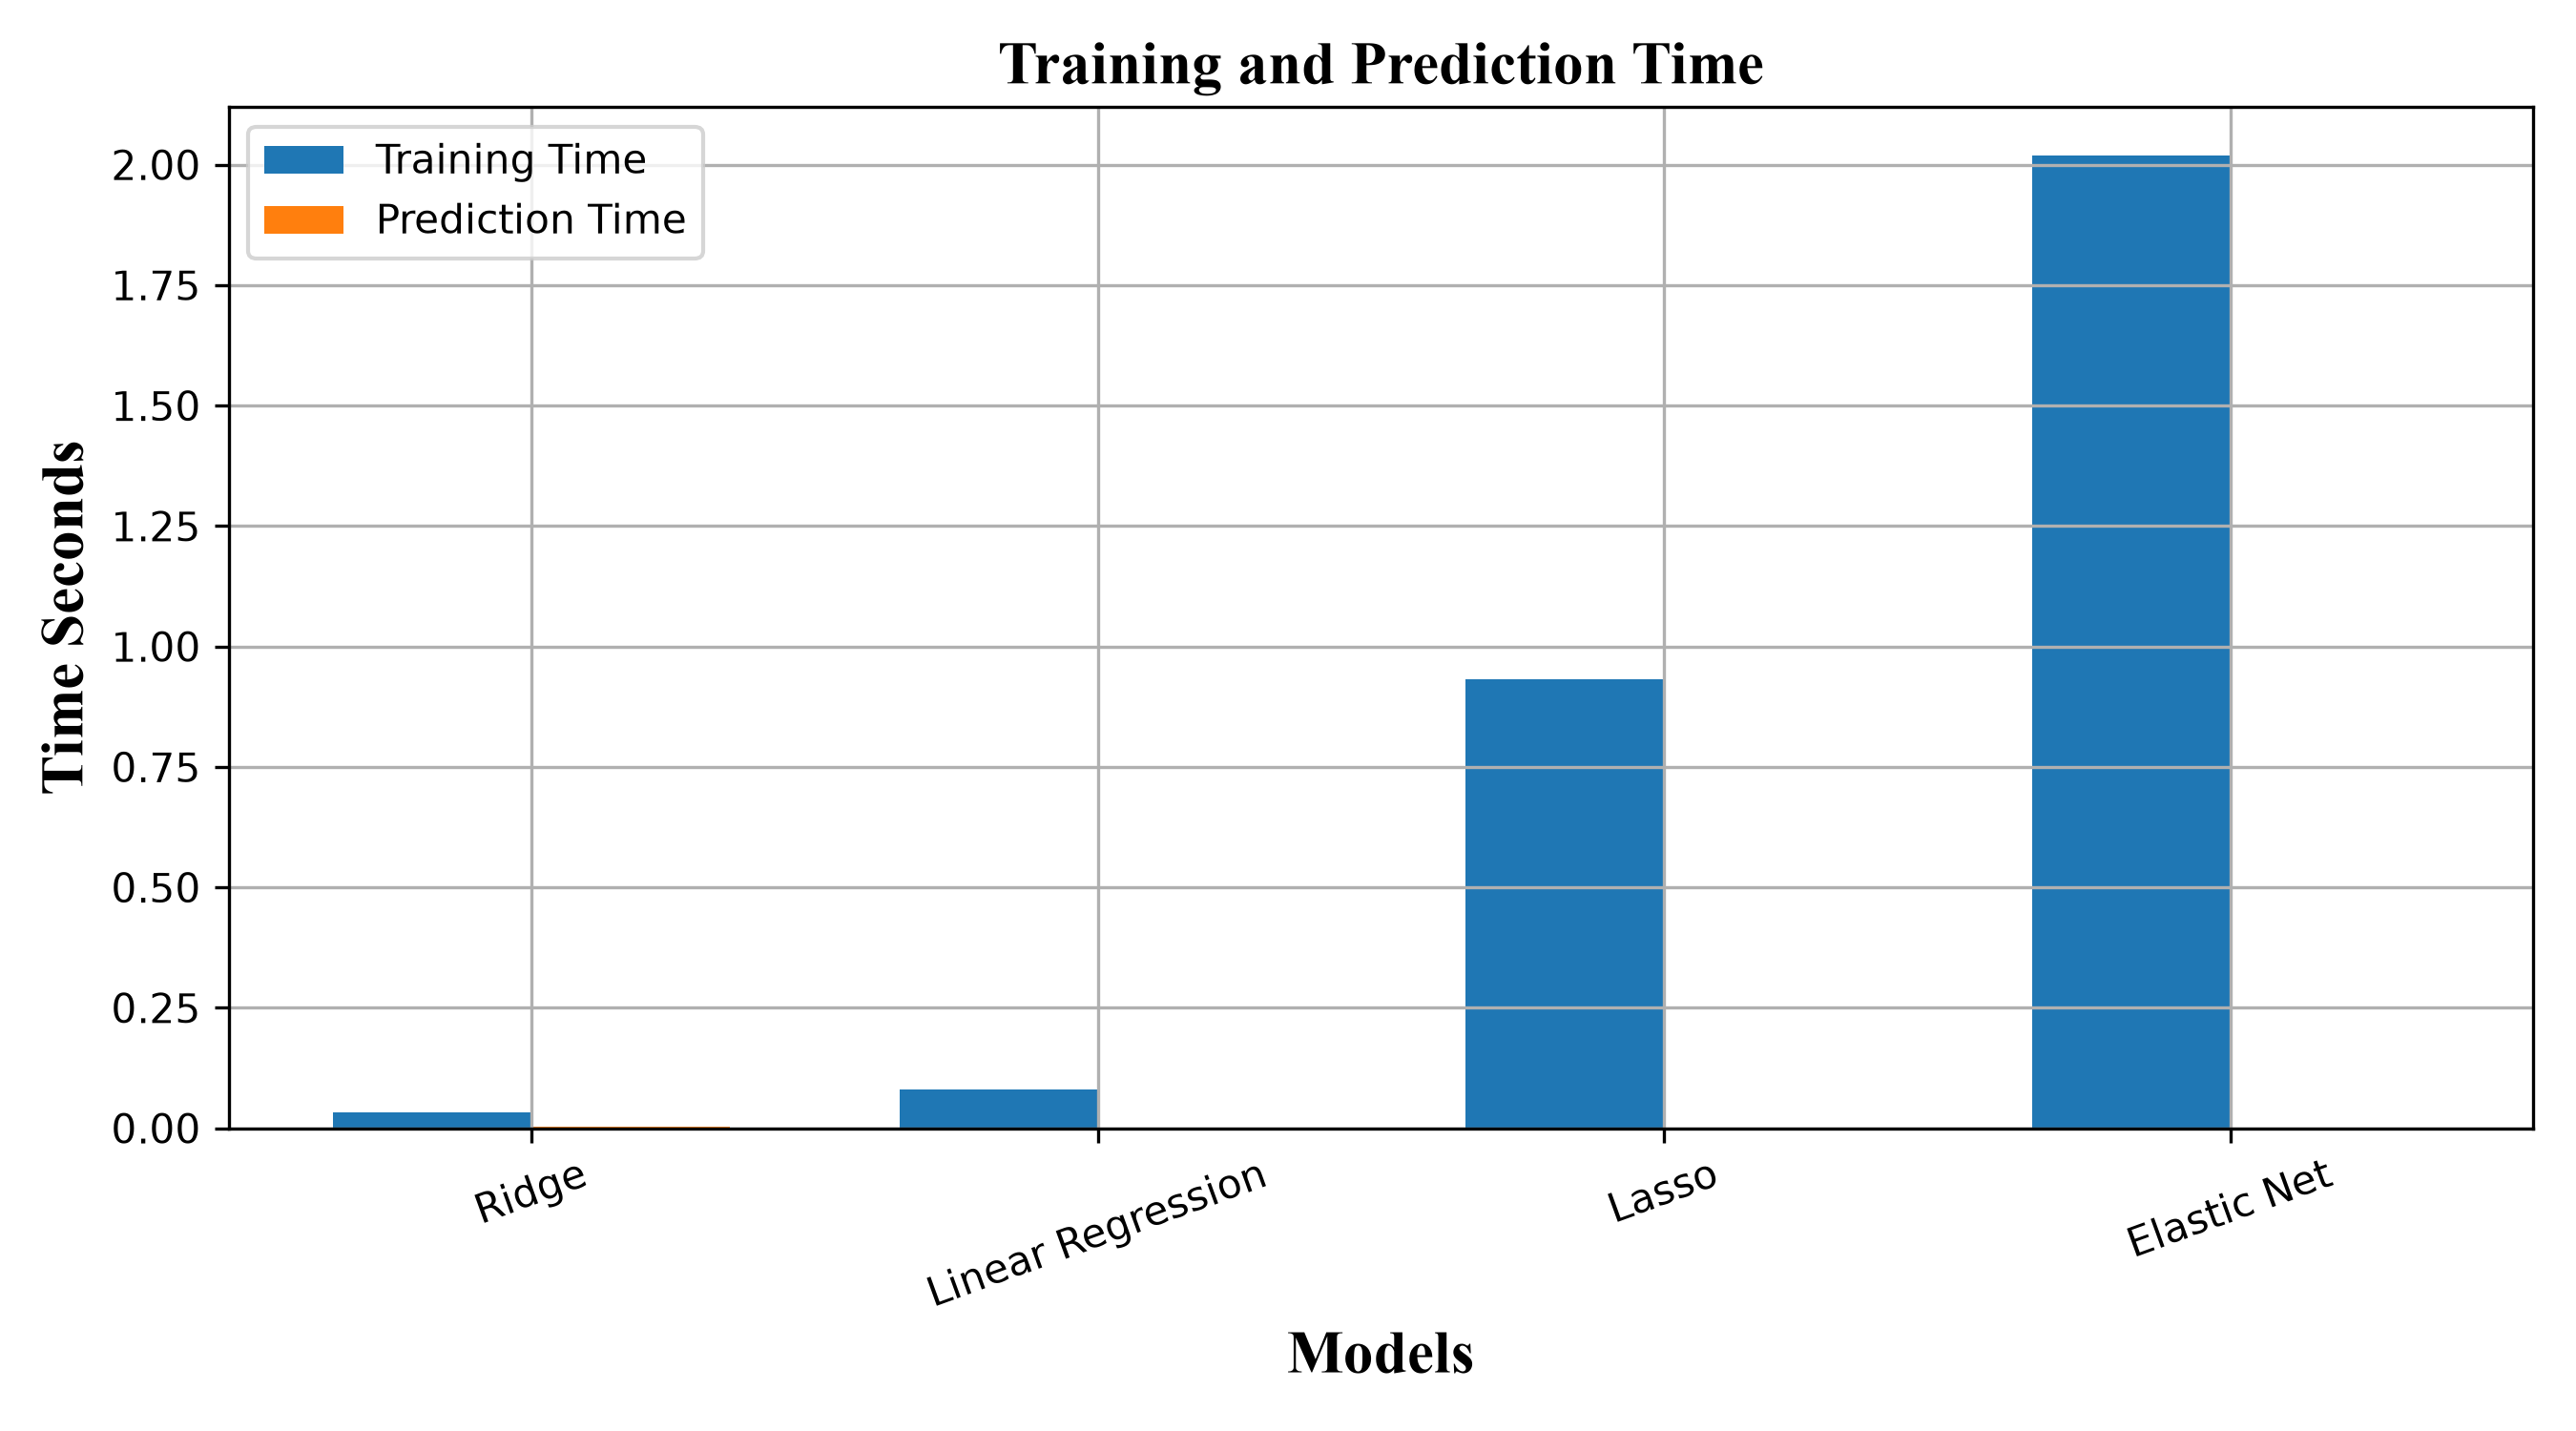
\includegraphics[width=0.7\linewidth]{training_prediction_time.png}
\caption{Training and Prediction Time Comparison (Bar Chart)}
\end{figure}

\textbf{Inference:} Ridge Regression required the least training time among all models (0.0186s), since its closed-form solution avoids the iterative coordinate-descent optimization required by L1-penalized models. Lasso and Elastic Net required substantially more training time (0.43s and 0.88s respectively) because their L1 terms are non-differentiable at zero and must be solved iteratively; Elastic Net is the slowest since it must jointly optimize both penalty terms. Prediction time was uniformly small (under 2ms) across all models, confirming that -- regardless of which model is chosen -- inference-time cost is negligible and would not be a deciding factor for real-time deployment. Training time, however, could matter for frequent model retraining pipelines, favoring Ridge or plain Linear Regression in that scenario.

\section{Overfitting and Underfitting Analysis}

The gap between training error and validation error was small across all four models (training MSE $\approx 9.39\times10^{8}$ vs. validation MSE $\approx 9.46$--$9.48\times10^{8}$), indicating that none of the models suffer from severe overfitting. Linear Regression, having no regularization, showed marginally larger coefficient magnitudes and slightly higher sensitivity to feature scale (particularly for Income), which is a mild indicator of variance relative to the regularized alternatives. Increasing regularization strength (higher $\alpha$ in Ridge, Lasso, and Elastic Net) reduced coefficient magnitude and stabilized validation error, confirming that regularization helped control variance without pushing the models into underfitting -- test and CV R$^2$ scores remained close to 0.60 throughout the entire hyperparameter search. No model showed clear signs of underfitting, since even the simplest Linear Regression baseline explained roughly 60\% of the variance in the target using only linear terms.

\section{Bias--Variance Analysis}

Linear Regression, being unregularized, has the lowest theoretical bias among the four models but is more susceptible to variance from correlated and outlier-heavy features such as Income and Property Age -- visible directly in its inflated Income coefficient (31491.86) relative to the regularized models. Ridge Regression reduces variance by shrinking all coefficients uniformly via the L2 penalty, trading a small increase in bias for improved stability, which is reflected in its consistent cross-validation performance (R$^2 = 0.5954$, very close to its test R$^2 = 0.6020$). Elastic Net further balances bias and variance by blending L1 and L2 penalties, which is particularly useful when features are correlated (e.g. Loan Amount Request and Property Price, correlation 0.726 and 0.687 respectively with the target, and likely correlated with each other). Lasso Regression introduces sparsity by driving several coefficients (e.g. Income) close to zero, increasing bias slightly for the features it effectively eliminates, but achieved the best overall variance reduction and generalization in this experiment, as shown by its top cross-validation and test R$^2$ scores -- suggesting that, for this dataset, the benefit of removing noisy/unstable features outweighs the small bias cost of doing so.

\section{Discussion}

The experiment implemented regression models for predicting loan sanction amounts using customer and property-related attributes. The dataset contained numerical and categorical features with a meaningful proportion of missing values (up to 24\% for Type of Employment), which were handled using mean imputation for numerical columns and mode imputation for categorical columns, following replacement of sentinel missing-value symbols (\texttt{-999}, \texttt{?}, \texttt{NA}, empty strings) with proper \texttt{NaN} markers. Categorical attributes were converted using one-hot encoding, and numerical features were standardized before model training to ensure fair treatment of features on different scales.

Four regression algorithms were compared:
\begin{itemize}
\item Linear Regression provided a strong, interpretable baseline model but showed signs of coefficient instability for outlier-prone features like Income.
\item Ridge Regression reduced coefficient magnitude using L2 regularization, improving stability with minimal loss in accuracy.
\item Lasso Regression performed explicit feature selection using L1 regularization, driving several low-signal coefficients toward zero.
\item Elastic Net combined both L1 and L2 penalties, offering a middle ground between Ridge's stability and Lasso's sparsity.
\end{itemize}

Among all models, Lasso Regression achieved the best test performance with an R$^2$ score of 0.6024 and the lowest RMSE of 29903.95. The results indicate that loan sanction amount depends mainly on the loan amount requested, property price, current loan expenses, and credit score, while demographic attributes such as age and number of dependents contribute comparatively little predictive power. This aligns with domain intuition: lenders base sanction decisions primarily on requested amount, collateral value, and creditworthiness rather than on personal or household characteristics.

A natural extension of this work -- noted here but outside the current scope -- would be to apply a log-transformation to heavily skewed features such as Income and the target variable itself, and to compare these linear models against non-linear alternatives (e.g. Decision Tree, Random Forest, or Gradient Boosting regressors) to check whether the residual $\sim$40\% of unexplained variance stems from genuine nonlinearity rather than noise.

\section{Conclusion}

This experiment successfully implemented regression analysis using Linear Regression and three regularized regression techniques -- Ridge, Lasso, and Elastic Net. The models were trained and evaluated using multiple performance metrics including MAE, MSE, RMSE, and R$^2$, and hyperparameter tuning using GridSearchCV with 5-fold cross-validation was used to identify optimal regularization strengths for each regularized model.

Lasso Regression achieved the best overall performance, with the highest test R$^2$ score (0.6024), the lowest RMSE (29903.95), and the highest cross-validation R$^2$ score (0.5957), and was therefore selected as the final regression model for loan sanction amount prediction. The experiment demonstrates that regularization techniques improve model stability -- particularly by controlling the influence of outlier-prone features such as Income -- and reduce unnecessary feature influence while maintaining, and in this case marginally improving, predictive accuracy relative to an unregularized baseline.

\section{References}

\begin{enumerate}
\item C. M. Bishop, \textit{Pattern Recognition and Machine Learning}, Springer, 2006.
\item T. Hastie, R. Tibshirani, and J. Friedman, \textit{The Elements of Statistical Learning}, 2nd ed., Springer, 2009.
\item S. Raschka and V. Mirjalili, \textit{Python Machine Learning}, 3rd ed., Packt Publishing, 2019.
\item F. Pedregosa et al., ``Scikit-learn: Machine Learning in Python,'' \textit{Journal of Machine Learning Research}, vol. 12, pp. 2825--2830, 2011.
\item Scikit-learn Documentation, \url{https://scikit-learn.org/}
\end{enumerate}

\section*{Appendix}

\subsection*{A.1 Implementation Details}

The experiment was implemented using Python with reusable modules for:
\begin{itemize}
\item Data preprocessing pipeline (\texttt{preprocessing.py})
\item Regression model training (\texttt{regression.py})
\item Hyperparameter optimization (\texttt{regression.py} -- \texttt{tune\_regression\_model()})
\item Cross validation (\texttt{validation.py})
\item Performance evaluation (\texttt{metrics.py})
\item Execution time benchmarking (\texttt{timing.py})
\item Visualization generation (\texttt{visualization.py}, \texttt{eda.py})
\end{itemize}

The implementation followed modular programming practices to improve code reusability and maintainability across experiments in this laboratory course.

\subsection*{A.2 Preprocessing Configuration Used}

\begin{lstlisting}
DROP_COLUMNS = [
    "Customer ID",
    "Name",
    "Property ID"
]

MISSING_VALUES = [
    "?",
    "-999",
    "",
    "NA"
]

X_train, X_test, y_train, y_test, preprocessor, feature_names = preprocess_data(
    df,
    TARGET,
    drop_cols=DROP_COLUMNS,
    missing_values=MISSING_VALUES,
    test_size=0.2
)
\end{lstlisting}

\subsection*{A.3 Final Tuned Hyperparameters}

\begin{lstlisting}
Ridge:        {'alpha': 100}
Lasso:        {'alpha': 10}
Elastic Net:  {'alpha': 0.1, 'l1_ratio': 0.8}
\end{lstlisting}

\end{document}